\makeatletter
\@ifundefined{standalonetrue}{\newif\ifstandalone}{}
\@ifundefined{section}{\standalonetrue}{\standalonefalse}
\makeatother
\ifstandalone
\documentclass{report}

\usepackage{textcase}
%\usepackage{hyperref}
%\hypersetup{breaklinks=true}


% Added packages
\usepackage[usenames]{color}
\usepackage{amsfonts, amsmath, amssymb, graphics}

% NOTE: bibentry MUST appear before the hyperref or build will fail
\usepackage{bibentry}
\nobibliography*
\usepackage[square,sort,comma,numbers]{natbib}
  
\usepackage{float}
\usepackage[
	hidelinks,%
    %hyperindex=true,		% Make numbers of index links as well
   	backref=page, 		% Provide page listing where refs occur in the bibliography
	%breaklinks=true,
    %colorlinks,%
    %citecolor=green,%
    %filecolor=blue,%
    %linkcolor=red,%
    %urlcolor=red, 
]{hyperref}

\usepackage{dsfont}
%%%% USEPACKAGES for MACROS %%%%%
\usepackage{algpseudocode}
\usepackage[chapter]{algorithm}
%\usepackage{caption}
\usepackage{subcaption}
\usepackage{url}

\usepackage{array}
\usepackage{arydshln}
\usepackage{multirow}
\usepackage{multicol}
%\usepackage[section]{placeins}

\usepackage[usenames,dvipsnames]{color}
%\usepackage[english]{babel}
\usepackage{tabularx}
\usepackage{soul}
\usepackage{xparse}
\usepackage{listings}
%\usepackage[normalem]{ulem}



%%%%%%%%%%%%%%%
% Show a list of items "todo" or "done" 
% USAGE: 
% \begin{todolist} 
% 	\todo Something not finished
% 	\done Something finished
% \end{todolist} 
\newenvironment{todolist}{%
  \begin{list}{}{}% whatever you want the list to be
  \let\olditem\item
  \renewcommand\item{\olditem \textcolor{red}{(TODO)}: }
  \newcommand\todo{\olditem \textcolor{red}{(TODO)}: }
   \newcommand\done{\olditem \textcolor{ForestGreen}{(DONE)}: }
}{%
  \end{list}
} 
%%%%%%%%%%%%%%%

%%%%%%%%%%%%%%%
% Show a Author's Note
% USAGE: 
% \incomplete[Optional footnote message to further clarify note]{The text which is currently not finished}
\DeclareDocumentCommand \incomplete{ o m }
{%
\IfNoValueTF {#1}
{\textcolor{red}{Incomplete: \ul{#2}}} 
{\textcolor{red}{Incomplete: \ul{#2}}\footnote{Comment: #1}}%
}
%%%%%%%%%%%%%%%



%%%%%%%%%%%%%%%
% Show a Author's Note
% USAGE: 
% \authnote[Optional footnote message to further clarify note]{The note to your readers}
\DeclareDocumentCommand \authnote { o m }
{%
\IfNoValueTF {#1}
{\textcolor{blue}{Author's Note: \ul{#2}}} 
{\textcolor{blue}{Author's Note: \ul{#2}}\footnote{Comment: #1}}%
}
%%%%%%%%%%%%%%%



%%%%%%%%%%%%%%%
% Strike out text that doesn't belong in the paper
% USAGE: 
% \strike[Optional footnote to state why it doesn't belong]{Text to strike out}
\DeclareDocumentCommand \strike { o m }
{%
\setstcolor{Red}
\IfNoValueTF {#1}
{\textcolor{Gray}{\st{#2}}} 
{\textcolor{Gray}{\st{#2}}\footnote{Comment: #1}}%
}
%%%%%%%%%%%%%%%

\definecolor{light-gray}{gray}{0.95}

\newcommand{\cbox}[3]{
\ \\
\fcolorbox{#1}{#2}{
\parbox{\textwidth}{
#3
}
}
}

% Setup an environment similar to verbatim but which will highlight any bash commands we have
\lstnewenvironment{unixcmds}[0]
{
%\lstset{language=bash,frame=shadowbox,rulesepcolor=\color{blue}}
\lstset{ %
language=sh,		% Language
basicstyle=\ttfamily,
backgroundcolor=\color{light-gray}, 
rulecolor=\color{blue},
%frame=tb, 
columns=fullflexible,
%framexrightmargin=-.2\textwidth,
linewidth=0.8\textwidth,
breaklines=true,
%prebreak=/, 
  prebreak = \raisebox{0ex}[0ex][0ex]{\ensuremath{\hookleftarrow}},
%basicstyle=\footnotesize,       % the size of the fonts that are used for the code
%numbers=left,                   % where to put the line-numbers
%numberstyle=\footnotesize,      % the size of the fonts that are used for the line-numbers
%stepnumber=2,                   % the step between two line-numbers. If it's 1 each line 
                                % will be numbered
%numbersep=5pt,                  % how far the line-numbers are from the code
showspaces=false,               % show spaces adding particular underscores
showstringspaces=false,         % underline spaces within strings
showtabs=false,                 % show tabs within strings adding particular underscores
frame=single,	                % adds a frame around the code
tabsize=2,	                % sets default tabsize to 2 spaces
captionpos=b,                   % sets the caption-position to bottom
breakatwhitespace=false,        % sets if automatic breaks should only happen at whitespace
}
} { }

% Setup an environment similar to verbatim but which will highlight any bash commands we have
\lstnewenvironment{cppcode}[1]
{
%\lstset{language=bash,frame=shadowbox,rulesepcolor=\color{blue}}
\lstset{ %
	backgroundcolor=\color{light-gray}, 
	rulecolor=\color[rgb]{0.133,0.545,0.133},
	tabsize=4,
	language=[GNU]C++,
%	basicstyle=\ttfamily,
        basicstyle=\scriptsize,
        upquote=true,
        aboveskip={1.5\baselineskip},
        columns=fullflexible,
        %framexrightmargin=-.1\textwidth,
       %framexleftmargin=6mm,
        showstringspaces=false,
        extendedchars=true,
        breaklines=true,
        prebreak = \raisebox{0ex}[0ex][0ex]{\ensuremath{\hookleftarrow}},
        frame=single,
        showtabs=false,
        showspaces=false,
        showstringspaces=false,
        numbers=left,                   % where to put the line-numbers
	numberstyle=\footnotesize,      % the size of the fonts that are used for the line-numbers
	stepnumber=4,                   % the step between two line-numbers. If it's 1 each line 
                                % will be numbered
	firstnumber=#1,
         numbersep=5pt,                  % how far the line-numbers are from the code
        identifierstyle=\ttfamily,
        keywordstyle=\color[rgb]{0,0,1},
        commentstyle=\color[rgb]{0.133,0.545,0.133},
        stringstyle=\color[rgb]{0.627,0.126,0.941},
}
} { }

% Setup an environment similar to verbatim but which will highlight any bash commands we have
\lstnewenvironment{mcode}[1]
{
\lstset{ %
	backgroundcolor=\color{light-gray}, 
	rulecolor=\color[rgb]{0.133,0.545,0.133},
	tabsize=4,
	language=Matlab,
%	basicstyle=\ttfamily,
        basicstyle=\scriptsize,
        upquote=true,
        aboveskip={1.5\baselineskip},
        columns=fullflexible,
        %framexrightmargin=-.1\textwidth,
       %framexleftmargin=6mm,
        showstringspaces=false,
        extendedchars=true,
        breaklines=true,
        prebreak = \raisebox{0ex}[0ex][0ex]{\ensuremath{\hookleftarrow}},
        frame=single,
        showtabs=false,
        showspaces=false,
        showstringspaces=false,
        numbers=left,                   % where to put the line-numbers
	numberstyle=\footnotesize,      % the size of the fonts that are used for the line-numbers
	stepnumber=4,                   % the step between two line-numbers. If it's 1 each line 
                                % will be numbered
	firstnumber=#1,
         numbersep=5pt,                  % how far the line-numbers are from the code
        identifierstyle=\ttfamily,
        keywordstyle=\color[rgb]{0,0,1},
        commentstyle=\color[rgb]{0.133,0.545,0.133},
        stringstyle=\color[rgb]{0.627,0.126,0.941},
}
} { }

\newcommand{\inputmcode}[1]{%
\lstset{ %
	backgroundcolor=\color{light-gray},  %
	rulecolor=\color[rgb]{0.133,0.545,0.133}, %
	tabsize=4, %
	language=Matlab, %
%	basicstyle=\ttfamily,
        basicstyle=\scriptsize, %
        %        upquote=true,
        aboveskip={1.5\baselineskip}, %
        columns=fullflexible, %
        %framexrightmargin=-.1\textwidth,
       %framexleftmargin=6mm,
        showstringspaces=false, %
        extendedchars=true, %
        breaklines=true, %
        prebreak = \raisebox{0ex}[0ex][0ex]{\ensuremath{\hookleftarrow}}, %
        frame=single, %
        showtabs=false, %
        showspaces=false, %
        showstringspaces=false,%
        numbers=left,                   % where to put the line-numbers
	numberstyle=\footnotesize,      % the size of the fonts that are used for the line-numbers
	stepnumber=4,                   % the step between two line-numbers. If it's 1 each line 
                                % will be numbered
         numbersep=5pt,                  % how far the line-numbers are from the code
        identifierstyle=\ttfamily, %
        keywordstyle=\color[rgb]{0,0,1}, %
        commentstyle=\color[rgb]{0.133,0.545,0.133}, %
        stringstyle=\color[rgb]{0.627,0.126,0.941} %
}
\lstinputlisting{#1}%
}

%\lstset{ %
%	backgroundcolor=\color{light-gray}, 
%	rulecolor=\color[rgb]{0.133,0.545,0.133},
%	tabsize=4,
%	language=Matlab,
%%	basicstyle=\ttfamily,
%        basicstyle=\scriptsize,
%        upquote=true,
%        aboveskip={1.5\baselineskip},
%        columns=fullflexible,
%        %framexrightmargin=-.1\textwidth,
%       %framexleftmargin=6mm,
%        showstringspaces=false,
%        extendedchars=true,
%        breaklines=true,
%        prebreak = \raisebox{0ex}[0ex][0ex]{\ensuremath{\hookleftarrow}},
%        frame=single,
%        showtabs=false,
%        showspaces=false,
%        showstringspaces=false,
%        numbers=left,                   % where to put the line-numbers
%	numberstyle=\footnotesize,      % the size of the fonts that are used for the line-numbers
%	stepnumber=4,                   % the step between two line-numbers. If it's 1 each line 
%                                % will be numbered
%	firstnumber=#1,
%         numbersep=5pt,                  % how far the line-numbers are from the code
%        identifierstyle=\ttfamily,
%        keywordstyle=\color[rgb]{0,0,1},
%        commentstyle=\color[rgb]{0.133,0.545,0.133},
%        stringstyle=\color[rgb]{0.627,0.126,0.941},
%}


\newcommand{\Laplacian}[1]{\nabla^2 #1}

% set of all nodes received and contained on GPU
\newcommand{\setAllNodes}[0]{\mathcal{G}}
% set of stencil centers on GPU
\newcommand{\setCenters}[0]{\mathcal{Q}}
% set of stencil centers with nodes in \setDepend
\newcommand{\setBoundary}[0]{\mathcal{B}}
% set of nodes received by other GPUs
\newcommand{\setDepend}[0]{\mathcal{R}}
% set of nodes sent to other GPUs
\newcommand{\setProvide}[0]{\mathcal{O}}


\newcommand{\toprule}[0]{\hline}
\newcommand{\midrule}[0]{\hline\hline}
\newcommand{\bottomrule}[0]{\hline}

\newcolumntype{C}{>{\centering\arraybackslash}b{1in}}
\newcolumntype{L}{>{\flushleft\arraybackslash}b{1.5in}}
\newcolumntype{R}{>{\flushright\arraybackslash}b{1.5in}}
\newcolumntype{D}{>{\flushright\arraybackslash}b{2.0in}}
\newcolumntype{E}{>{\flushright\arraybackslash}b{1.0in}}

\DeclareSymbolFont{AMSb}{U}{msb}{m}{n}
\DeclareMathSymbol{\N}{\mathbin}{AMSb}{"4E}
\DeclareMathSymbol{\Z}{\mathbin}{AMSb}{"5A}
\DeclareMathSymbol{\R}{\mathbin}{AMSb}{"52}
\DeclareMathSymbol{\Q}{\mathbin}{AMSb}{"51}
\DeclareMathSymbol{\PP}{\mathbin}{AMSb}{"50}
\DeclareMathSymbol{\I}{\mathbin}{AMSb}{"49}
%\DeclareMathSymbol{\C}{\mathbin}{AMSb}{"43}

%%%%%% VECTOR NORM: %%%%%%%
\newcommand{\vectornorm}[1]{\left|\left|#1\right|\right|}
\newcommand{\vnorm}[1]{\left|\left|#1\right|\right|}
\newcommand{\by}[0]{\times}
\newcommand{\vect}[1]{\mathbf{#1}}
%\newcommand{\mat}[1]{\mathbf{#1}} 

%\renewcommand{\vec}[1]{ \textbf{#1} }
%%%%%%%%%%%%%%%%%%%%%%

%%%%%%% THM, COR, DEF %%%%%%%
%\newtheorem{theorem}{Theorem}[section]
%\newtheorem{lemma}[theorem]{Lemma}
%\newtheorem{proposition}[theorem]{Proposition}
%\newtheorem{corollary}[theorem]{Corollary}
%\newenvironment{proof}[1][Proof]{\begin{trivlist}
%\item[\hskip \labelsep {\bfseries #1}]}{\end{trivlist}}
%\newenvironment{definition}[1][Definition]{\begin{trivlist}
%\item[\hskip \labelsep {\bfseries #1}]}{\end{trivlist}}
%\newenvironment{example}[1][Example]{\begin{trivlist}
%\item[\hskip \labelsep {\bfseries #1}]}{\end{trivlist}}
%\newenvironment{remark}[1][Remark]{\begin{trivlist}
%\item[\hskip \labelsep {\bfseries #1}]}{\end{trivlist}}
%\newcommand{\qed}{\nobreak \ifvmode \relax \else
%      \ifdim\lastskip<1.5em \hskip-\lastskip
%      \hskip1.5em plus0em minus0.5em \fi \nobreak
%      \vrule height0.75em width0.5em depth0.25em\fi}
%%%%%%%%%%%%%%%%%%%%%%

%
%\usepackage[algochapter]{algorithm2e}
%\usepackage[usenames]{color}
% colors to show the corrections
\newcommand{\red}[1]{\textbf{\textcolor{red}{#1}}}
\newcommand{\blue}[1]{\textbf{\textcolor{blue}{#1}}}
\newcommand{\cyan}[1]{\textbf{\textcolor{cyan}{#1}}}
\newcommand{\green}[1]{\textbf{\textcolor{green}{#1}}}
\newcommand{\magenta}[1]{\textbf{\textcolor{magenta}{#1}}}
\newcommand{\orange}[1]{\textbf{\textcolor{orange}{#1}}}
%%%%%%%%%% DK DK
% comments between authors
\newcommand{\toall}[1]{\textbf{\green{@@@ All: #1 @@@}}}
\newcommand{\toevan}[1]{\textbf{\red{*** Evan: #1 ***}}}
%\newcommand{\toevan}[1]{}  % USE FOR FINAL VERSION
\newcommand{\toe}[1]{\textbf{\red{*** Evan: #1 ***}}}
\newcommand{\tog}[1]{\textbf{\blue{*** Gordon: #1 ***}}}
%\newcommand{\togordon}[1]{\textbf{\blue{*** Gordon: #1 ***}}}
\renewcommand{\ge}[3]{{\textcolor{blue}{*** \textbf{Gordon:}\strike{#1} #2 ***}}\red{(#3)}}
\renewcommand{\ge}[3]{{\textcolor{blue}{#2}}}
\renewcommand{\ge}[3]{{\textcolor{Red}{#2}}}
\newcommand{\eb}[3]{{\textcolor{Red}{*** \textbf{Evan:}\strike{#1} #2 ***}}\red{(#3)}}
\renewcommand{\eb}[3]{{{\textcolor{Red}{#2}}}}
%\def\ge#1#2#3{}{\textbf{\blue{*** Gordon: #2 ***}}}{(#3)}
\newcommand{\gee}[1]{{\bf{\blue{{\em #1}}}}}
\newcommand{\old}[1]{}
\newcommand{\del}[1]{***#1*** }



% \DeclareMathOperator{\Sample}{Sample}
%\let\vaccent=\v % rename builtin command \v{} to \vaccent{}
%\renewcommand{\vec}[1]{\ensuremath{\mathbf{#1}}} % for vectors
\newcommand{\gv}[1]{\ensuremath{\mbox{\boldmath$ #1 $}}} 
% for vectors of Greek letters
\newcommand{\uv}[1]{\ensuremath{\mathbf{\hat{#1}}}} % for unit vector
\newcommand{\abs}[1]{\left| #1 \right|} % for absolute value
\newcommand{\avg}[1]{\left< #1 \right>} % for average
\let\underdot=\d % rename builtin command \d{} to \underdot{}
\renewcommand{\d}[2]{\frac{d #1}{d #2}} % for derivatives
\newcommand{\dd}[2]{\frac{d^2 #1}{d #2^2}} % for double derivatives
\newcommand{\pd}[2]{\frac{\partial #1}{\partial #2}} 
% for partial derivatives
\newcommand{\pdd}[2]{\frac{\partial^2 #1}{\partial #2^2}} 
\newcommand{\pdda}[3]{\frac{\partial^2 #1}{\partial #2 \partial #3}} 
% for double partial derivatives
\newcommand{\pdc}[3]{\left( \frac{\partial #1}{\partial #2}
 \right)_{#3}} % for thermodynamic partial derivatives
\newcommand{\ket}[1]{\left| #1 \right>} % for Dirac bras
\newcommand{\bra}[1]{\left< #1 \right|} % for Dirac kets
\newcommand{\braket}[2]{\left< #1 \vphantom{#2} \right|
 \left. #2 \vphantom{#1} \right>} % for Dirac brackets
\newcommand{\matrixel}[3]{\left< #1 \vphantom{#2#3} \right|
 #2 \left| #3 \vphantom{#1#2} \right>} % for Dirac matrix elements
\newcommand{\grad}[1]{\gv{\nabla} #1} % for gradient
\let\divsymb=\div % rename builtin command \div to \divsymb
\renewcommand{\div}[1]{\gv{\nabla} \cdot #1} % for divergence
\newcommand{\curl}[1]{\gv{\nabla} \times #1} % for curl
\let\baraccent=\= % rename builtin command \= to \baraccent
\renewcommand{\=}[1]{\stackrel{#1}{=}} % for putting numbers above =
\newcommand{\diffop}[1]{\mathcal{L}#1}
\newcommand{\boundop}[1]{\mathcal{B}#1}
\newcommand{\rvec}[0]{{\bf r}}

\newcommand{\Interior}[0]{\Omega}
\newcommand{\domain}[0]{\Omega}
%\newcommand{\Boundary}[0]{\partial \Omega}
\newcommand{\Boundary}[0]{\Gamma}

\newcommand{\on}[1]{\hskip1.5em \textrm{ on } #1}

\newcommand{\gemm}{\texttt{GEMM}}
\newcommand{\trmm}{\texttt{TRMM}}
\newcommand{\gesvd}{\texttt{GESVD}}
\newcommand{\geqrf}{\texttt{GEQRF}}


\newcommand{\minitab}[2][l]{\begin{tabular}{#1}#2\end{tabular}}
\newcommand{\comm}[1]{\textcolor{red}{\textit{#1}}}

\newcommand{\nfrac}[2]{
\nicefrac{#1}{#2}
%\frac{#1}{#2}
}

\usepackage{xparse}
\usepackage{soul}


%%%%%%%%%%%%%%%
% Show a Author's Note
% USAGE: 
% \incomplete[Optional footnote message to further clarify note]{The text which is currently not finished}
\DeclareDocumentCommand \incomplete{ o m }
{%
\IfNoValueTF {#1}
{\textcolor{red}{Incomplete: \ul{#2}}} 
{\textcolor{red}{Incomplete: \ul{#2}}\footnote{Comment: #1}}%
}
%%%%%%%%%%%%%%%



%%%%%%%%%%%%%%%
% Show a Author's Note
% USAGE: 
% \authnote[Optional footnote message to further clarify note]{The note to your readers}
\DeclareDocumentCommand \authnote { o m }
{%
\IfNoValueTF {#1}
{\textcolor{blue}{Author's Note: \ul{#2}}} 
{\textcolor{blue}{Author's Note: \ul{#2}}\footnote{Comment: #1}}%
}
%%%%%%%%%%%%%%%



%%%%%%%%%%%%%%%
% Strike out text that doesn't belong in the paper
% USAGE: 
% \strike[Optional footnote to state why it doesn't belong]{Text to strike out}
\DeclareDocumentCommand \strike { o m }
{%
\setstcolor{red}
\IfNoValueTF {#1}
{\textcolor{Gray}{\st{#2}}} 
{\textcolor{Gray}{\st{#2}}\footnote{Comment: #1}}%
}
%%%%%%%%%%%%%%%



%
% colors to show the corrections
\newcommand{\red}[1]{\textbf{\textcolor{red}{#1}}}
\newcommand{\blue}[1]{\textbf{\textcolor{blue}{#1}}}
\newcommand{\cyan}[1]{\textbf{\textcolor{cyan}{#1}}}
\newcommand{\green}[1]{\textbf{\textcolor{green}{#1}}}
\newcommand{\magenta}[1]{\textbf{\textcolor{magenta}{#1}}}
\newcommand{\orange}[1]{\textbf{\textcolor{orange}{#1}}}
%%%%%%%%%% DK DK
% comments between authors
\newcommand{\toall}[1]{\textbf{\green{@@@ All: #1 @@@}}}
\newcommand{\toevan}[1]{\textbf{\red{*** Evan: #1 ***}}}
%\newcommand{\toevan}[1]{}  % USE FOR FINAL VERSION
\newcommand{\toe}[1]{\textbf{\red{*** Evan: #1 ***}}}
\newcommand{\tog}[1]{\textbf{\blue{*** Gordon: #1 ***}}}
%\newcommand{\togordon}[1]{\textbf{\blue{*** Gordon: #1 ***}}}
\renewcommand{\ge}[3]{{\textcolor{blue}{*** \textbf{Gordon:}\strike{#1} #2 ***}}\red{(#3)}}
\renewcommand{\ge}[3]{{\textcolor{blue}{#2}}}
\renewcommand{\ge}[3]{{\textcolor{red}{#2}}}
\newcommand{\eb}[3]{{\textcolor{red}{*** \textbf{Evan:}\strike{#1} #2 ***}}\red{(#3)}}
\renewcommand{\eb}[3]{{{\textcolor{red}{#2}}}}
%\def\ge#1#2#3{}{\textbf{\blue{*** Gordon: #2 ***}}}{(#3)}
\newcommand{\gee}[1]{{\bf{\blue{{\em #1}}}}}
\newcommand{\old}[1]{}
\newcommand{\del}[1]{***#1*** }



% Rename  this file          misc_mac.tex
%----------------------------------------------------------------------
%%%%%%%%%%%%%%%%%%%%%%%%%%%%%%%%%%%%%%%%%%%%%%%%%%%%%%%%%%%%%%%%%%%%%%%%%%%%%%%
%
%	Math Symbols   Math Symbols   Math Symbols   Math Symbols   
%
%%%%%%%%%%%%%%%%%%%%%%%%%%%%%%%%%%%%%%%%%%%%%%%%%%%%%%%%%%%%%%%%%%%%%%%%%%%%%%%
\def\pmb#1{\setbox0=\hbox{$#1$}%
	\kern-.025em\copy0\kern-\wd0
	\kern.05em\copy0\kern-\wd0
	\kern-.025em\raise.0433em\box0}
\def\pmbf#1{\pmb#1}
\def\bfg#1{\pmb#1}

% BETTER VALUES FOR AUTOMATIC FIGURE PLACEMENT THAN THOSE PROVIDED BY 
% LATEX DEFAULTS.

\renewcommand{\textfloatsep}{1ex}
\renewcommand{\floatpagefraction}{0.9}
\renewcommand{\intextsep}{1ex}
\renewcommand{\topfraction}{.9}
\renewcommand{\bottomfraction}{.9}
\renewcommand{\textfraction}{.1}

% #1  position of floating figure (h|t|b|p)
% #1  EPS postscript file
% #2  size
% #3  caption

%usage of newfig:
%  \newfig{file.ps}{3in}{Fig1: this is a figure}

\input{epsf}
\def\newfig#1#2#3{
  \begin{figure}[htbp]
  \vspace{1ex}
  \setlength{\epsfxsize}{#2}
  \centerline{\epsfbox{#1}}
  \vspace{-.1in}\caption{\small #3}\break\vspace{.2in}
  \label{#1}
  \end{figure}
}

%usage of newfigtwo: 2 figures, vertically stacked
% \newfig
%	{file1.ps}
%	{file2.ps}
%	{width}
%	{vertical space}
%	{Caption}

\def\newfigtwo#1#2#3#4#5{
  \begin{figure}[htbp]
  \vspace{1ex}
  \setlength{\epsfxsize}{#3}
  \centerline{\epsfbox{#1}}
  \vspace{#4}
  \setlength{\epsfxsize}{#3}
  \centerline{\epsfbox{#2}}
  \vspace{-.1in}\caption{\small #5}\break\vspace{.2in}
  \label{#1}
  \end{figure}
}

\def\newfigh#1#2#3#4{  % add height specification
  \begin{figure}[htbp]
  \vspace{1ex}
  \setlength{\epsfxsize}{#2}
  \setlength{\epsfysize}{#4}
  \centerline{\epsfbox{#1}}
  \vspace{-.1in}\caption{\small #3}\break\vspace{.2in}
  \label{#1}
  \end{figure}
}

\def\herefig#1#2#3{
  \begin{figure}[h]
  \setlength{\epsfxsize}{#2}
  \centerline{\epsfbox{#1}}
  \caption{\small #3}
  \label{#1}
  \end{figure}
}

\def\etal{{{\em et~al.\,\,}}}
\def\note#1{\\ =====#1===== \\}
\def\FBOX#1{\ \\ \fbox{\begin{minipage}{5in}#1\end{minipage}}\\ }
\newcount\sectionno     \sectionno=0
\newcount\eqnum         \eqnum=0
\def\addeqno{\global\advance \eqnum by  1 }
\def\subeqno{\global\advance \eqnum by -1 }
%\def\eqn{\addeqno \eqno \hbox{(\number\sectionno.\number\eqnum)} }

\def\tildetilde#1{\tilde{\tilde{#1}}}
\def\barbar#1{\overbar{\overbar{#1}}}

\def\vsp#1{\vspace{#1 ex}}
\def\fpar{\hspace{\parindent}}
%
%  \pf : 2 arguments: numerator and denominator of partial derivative
%
\def\pf#1#2{{\frac{\partial{#1}}{\partial{#2}}}}
\def\pfs#1#2{{\partial_{#2}{#1}}}
\def\pftwo#1#2{{\frac{\partial^2{#1}}{\partial{#2}^2}}}
\def\pfxx#1#2{{\frac{\partial^2{#1}}{\partial{#2}^2}}}
%\def\pfxy#1#2{{\frac{\partial^2{#1}}{\partial{#2}\partial{#3}}}}
\def\pfn#1#2#3{{\frac{\partial^{#1}{#2}}{\partial{#3}^{#1}}}}
\def\df#1#2{{\frac{d{#1}}{d{#2}}}}
\def\dfn#1#2#3{{\frac{d^{#1}{#2}}{d{#3}^{#1}}}}
\def\Dt#1#2{\frac{D#1}{D#2}}
\def\dt#1#2{\frac{d#1}{d#2}}
\def\bld#1{{\bf #1}}
\def\pfp#1#2#3{\pf{}{#3}{\left(\frac{#1}{#2}\right)}}

\def\norm#1{\|#1\|}

%
% Graphic characters  (\dot already defined by TeX/LateX)
%
\def\dash{\rule[1.5pt]{2mm}{.3mm}\HS{.9mm}}
\def\dott{\rule[1.5pt]{.7mm}{.3mm}\HS{.7mm}}
\def\dashline{\dash\dash\dash}
\def\dotline{\dott\dott\dott\dott\dott\dott}
\def\dashdotline{\dash$\cdot$\HS{.9mm}\dash}
\def\solidline{\rule[2pt]{7mm}{.3mm}}
% 
% overcircle
%
\def\ovcircle#1{\buildrel{\circ}\over{#1}}
%\def\below#1#2{\buildrel{#2}\under{#1}}
%\def\above#1#2{\buildrel{#2}\over{#1}}
%
%  big parenthesis and brackets
%
\def\bigpar#1#2{{\left(\frac{#1}{#2}\right)}}
\def\bigbra#1#2{{\left\[\frac{#1}{#2}\right\]}}

\def\Lp{\left(}
\def\Rp{\right)}
\def\Lb{\left[}
\def\Rb{\right]}
\def\Ln{\left\langle}
\def\Rn{\right\rangle}
\def\Ld{\left.}
\def\Rd{\right.}
\def\Lv{\left|}
\def\Rv{\right|}
\def\Lbr{\left|}
\def\Rbr{\right|}
\def\lng{\langle}
\def\rng{\rangle}
\def\Lc{\left\{}
\def\Rc{\right\}}
%%% %

% Cannot be handled by Lyx
%\def\[{{[}}
%\def\]{{]}}

%
\def\eol{\nonumber \\}
\def\eolnonb{\nonumber\\}
\def\eolnb{\\}
\def\nonb{\nonumber}
\def\be{\begin{equation}}
\def\ee{\end{equation}}
\def\BEQNA{\begin{eqnarray}}
\def\EEQNA{\end{eqnarray}}
\def\eqa{&=&}
\def\beqna{\begin{eqnarray}}
\def\eeqna{\end{eqnarray}}
\def\bverb{\begin{verbatim}}
\def\everb{\end{verbatim}}
\def\VERB#1{\bverb #1 \everb}
\def\btbl{\begin{tabular}}
\def\etbl{\end{tabular}}
\def\bmini{\begin{minipage}[t]{5.5in}}
\def\emini{\end{minipage}}
\def\parray#1#2{\left(\begin{array}{#1}#2\end{array}\right)}
\def\barray#1#2{\left[\begin{array}{#1}#2\end{array}\right]}
\def\carray#1#2{\left\{\begin{array}{#1}#2\end{array}\right.}
\def\darray#1#2{\left|\begin{array}{#1}#2\end{array}\right|}

\def\BEGTABLE#1{\begin{table}[hbt]\vspace{2ex}\begin{center}\bmini\centering\btbl{#1}}
\def\ENDTABLE#1#2{\etbl\caption[#1]{#2}\EMINI\end{center}\vspace{2ex}\end{table}}

\def\bfltbl#1{\begin{table}[hbt]\vspace{2ex}\begin{center}\bmini\centering\btbl{#1}}
\def\efltbl#1#2{\etbl\caption[#1]{#2}\emini\end{center}\vspace{2ex}\end{table}}
\def\mcol{\multicolumn}
%
%  label equations with (#)
%
\def\reff#1{(\ref{#1})}
%
%  macros borrowed from viewgraph package
%

\newenvironment{LETTRS}[3]{\begin{letter}{#1}
\input{origin}\opening{Dear #2:}\input{#3}\closing{Sincerely yours,}\end{letter}}{\clearpage}

\newenvironment{VIEW}[1]{{\BC\Huge\bf #1 \EC}\LARGE\VS{.05in}}{\clearpage}

\def\RM#1{\rm{#1\ }}
\def\BV{\begin{VIEW}}
\def\EV{\end{VIEW}}

\def\NI{\noindent}

\def\VS{\vspace*}
\def\HS{\hspace*}
\def\IT{\item}

\def\BARR{\begin{array}}
\def\EARR{\end{array}}

\def\BPARR{\left(\begin{array}}
\def\EPARR{\end{array}\right)}

\def\BDET{\left|\begin{array}}
\def\EDET{\end{array}\right|}

\def\BDF{\begin{definition}}
\def\EDF{\end{definition}}

\def\BSU{\begin{block}{Summary}}
\def\ESU{\end{block}}

\def\BEX{\begin{example}}
\def\EEX{\end{example}}

\def\BTH{\begin{theorem}}
\def\ETH{\end{theorem}}

\def\BCO{\begin{corollary}}
\def\ECO{\end{corollary}}

\def\BPROOF{\begin{proof}}
\def\EPROOF{\end{proof}}

\def\BLM{\begin{lemma}}
\def\ELM{\end{lemma}}

\def\BEQ{\begin{equation}}
\def\EEQ{\end{equation}}

\def\BEQNNB{$$}
\def\EEQNNB{$$}

\def\BE{\begin{enumerate}}
\def\EE{\end{enumerate}}

\def\BD{\begin{description}}
\def\ED{\end{description}}

\def\BI{\begin{itemize}}
\def\EI{\end{itemize}}

\def\BC{\begin{center}}
\def\EC{\end{center}}

\def\BFIG{\begin{figure}}
\def\EFIG{\end{figure}}

\def\BTABB{\begin{tabbing}}
\def\ETABB{\end{tabbing}}

\def\BMINI{\begin{minipage}}
\def\EMINI{\end{minipage}}

\def\BTABLE{\begin{table}}
\def\ETABLE{\end{table}}

\def\BTABUL{\begin{tabular}}
\def\ETABUL{\end{tabular}}

\def\MCOL{\multicolumn}
\def\UL{\underline}
\def\ULL#1{\UL{\UL{#1}}}

\def\BDOC{\begin{document}}
\def\EDOC{\end{document}}

\def\EM#1{{\em #1\/}}
\def\FN{\footnote}

% Courtesy of Ugo Piomelli

\def\latexfig #1 #2 #3 #4 #5 {\ \vfill
\hfill\hbox to 0.05in{\vbox to #3truein{
         \special{psfile="#1" angle=270 hscale=100 
                  hoffset=#4 voffset=#5 vscale=100} }\hfill}
\hfill\vspace{-0.1in}        }

% #1 is the .ps filename
% #2 is not used in the present version
% #3 is the size of the white space left above the caption (in inches)
% #4 is the horizontal offset from some unknown reference point.
%    It is in 1/72 of an inch and is positive to the right.
% #5 is the vertical offset from some unknown reference point.
%    It is in 1/72 of an inch and is positive upwards.


\newcommand{\mathsym}[1]{{}}
\newcommand{\unicode}[1]{{}}
\newcommand{\ep}{\epsilon}
\newcommand{\vv}{\mathbf{v}}
\newcommand{\vu}{\mathbf{u}}
\newcommand{\vx}{\mathbf{x}}

\newcommand{\Laplacian}[1]{\nabla^2 #1}
\newcommand{\LaplaceBeltrami}[1]{\Delta_S #1}

% set of all nodes received and contained on GPU
\newcommand{\setAllNodes}[0]{\mathcal{G}}
% set of stencil centers on GPU
\newcommand{\setCenters}[0]{\mathcal{Q}}
% set of stencil centers with nodes in \setDepend
\newcommand{\setBoundary}[0]{\mathcal{B}}
% set of nodes received by other GPUs
\newcommand{\setDepend}[0]{\mathcal{R}}
% set of nodes sent to other GPUs
\newcommand{\setProvide}[0]{\mathcal{O}}





\usepackage{tabularx} 
\newcolumntype{C}{>{\centering\arraybackslash}b{1in}}
\newcolumntype{L}{>{\flushleft\arraybackslash}b{1.5in}}
\newcolumntype{R}{>{\flushright\arraybackslash}b{1.5in}}
\newcolumntype{D}{>{\flushright\arraybackslash}b{2.0in}}
\newcolumntype{E}{>{\flushright\arraybackslash}b{1.0in}}


 


%\usepackage{xcolor}

%\usepackage{refcheck}
% Sepia
%\definecolor{myBGcolor}{HTML}{F6F0D6}
%\definecolor{myTextcolor}{HTML}{4F452C}
% Dark
%\definecolor{myBGcolor}{HTML}{3E3535}
%\definecolor{myTextcolor}{HTML}{CFECEC}
%\color{myTextcolor}
%\pagecolor{myBGcolor}
 

\begin{document}
\fi




\chapter{An Alternative Stencil Generation Algorithm for RBF-FD}
\label{chap:stencils}

Like all RBF methods, RBF-FD is designed to handle irregular node distributions, so the emphasis in literature focuses on how the method manages point clouds. While nothing prevents implementations of RBF-FD from utilizing existing meshes/lattices, most work in the field concentrates on simple geometries to better understand properties of the method and develop extensions. Without mesh/lattice connectivity available, stencils are generated by choosing the $n$-nearest neighbors to a center node, inclusive of the center. This is known more formally as a \emph{$k$-nearest neighbor (k-NN)} problem \cite{TagliasacchiMFE} (a.k.a. $\ell$-nearest neighbor search \cite{WendlandBook}). Here ``nearest" is defined with the Euclidean distance metric, although it is possible to generalize to other metrics (see e.g., \cite{MatlabKDTreeSearcher}). 

In comparison to the RBF-FD method, global RBF methods with infinite support connect all nodes to all other nodes, so there is no need for neighbor queries. On the other hand, compact RBF methods require all nodes---with no limit on the count---that lie within the support/radius of the RBF centered at each node. This type of neighbor query is referred to as a \emph{ball query} (a.k.a. range query \cite{WendlandBook}) due to the closed ball created by the radius of support for a compact RBF (see Equation~\ref{eqn:csrbf}). 

The $k$-NN and ball query share many similarities, but the former can be harder to solve. Consider, for example, the scenario in Figure~\ref{fig:nearest_neighbor_example}. Two ball queries around a green stencil center are represented as dashed and dash-dot circles. The inner query returns four neighbors, and the outer returns six. If a stencil of size $n=6$ is desired, then the outer query can be truncated to give the five required neighbors shown in blue. In this example the red node and the farthest blue node are equidistant from the center, and ties are broken arbitrarily. Although $k$-NN is simply a truncated ball query, the real challenge lies in finding the proper search radius to enclose at least the $n$ desired neighbors. To find the radius in practice depends on the choice of data structure used to access node locations. 

\begin{figure}
\centering
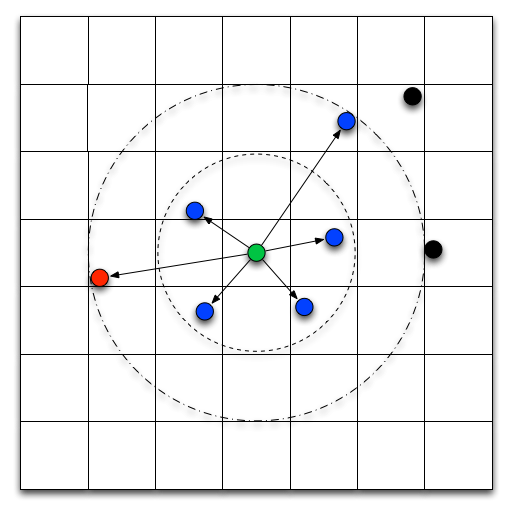
\includegraphics[width=5.5cm]{rbffd_methods_content/neighbors/ball_query_vs_kNN.png}
\caption{A stencil center in green finds neighboring stencil nodes in blue. Two ball queries are shown as dashed and dash-dot circles to demonstrate the added difficulty of finding the right query radius to obtain the $k$-nearest neighbors.}
\label{fig:nearest_neighbor_example}
\end{figure}


A na\"{i}ve approach for neighbor queries would be a brute-force search that checks distances from all nodes to every other node. Obviously the cost of such a method is high: $O(N^2)$ for all stencils. Multi-dimensional data structures, such as those discussed here, can limit the scope of searching and reduce the cost of stencil generation to $O(N \log{N})$. 

For the most part, investigations in RBF communities that delve into efficient neighbor queries are limited to ball queries. For example, the Partition of Unity method for approximation (e.g., \cite{Wendland2002,WendlandBook}), and particle methods like the Fast Multipole Method (e.g., \cite{Ying2006, Gumerov2003}) or Smoothed Particle Hydrodynamics (e.g., \cite{Krog2010}). Examples of fast algorithms employed in these fields include the fixed-grid method \cite{WendlandBook,Krog2010}, $k$-D Trees \cite{WendlandBook}, Range Trees \cite{Wendland2002,WendlandBook}, and $2^d$-Trees (i.e., Quad- and Octrees) \cite{Gumerov2003, Ying2006}. Surprisingly, while other communities continue the quest for fast neighbor queries, RBF collocation and RBF-FD communities have been slow on the uptake. For many years, the standard in the community has been to use $k$-D Trees (see e.g., \cite{Fasshauer2007, FlyerLehto11,FornbergLehto11}). 


This chapter considers the use of an alternative neighbor query algorithm to generate RBF-FD stencils. It is based loosely on the fixed-grid method from \cite{Krog2010,Green2010,Johnson2011}. \cite{Samet2005} would classify the algorithm as a \emph{fixed grid ``bucket" method with one-dimensional spatial ordering}. The fixed-grid method loosens the requirements for finding the $k$-nearest neighbors ($k$-NN) stencils to accept $k$-``approximately nearest" neighbors ($k$-ANN). It also reorders nodes according to space-filling curves. In what follows, the fixed-grid method is compared to an efficient implementation of $k$-D Tree available for use in C++ and MATLAB (\cite{TagliasacchiMFE}). Benchmarks demonstrate that, with the proper choice of parameters for the fixed-grid, the method is up to 2x faster than $k$-D Tree, and it comes with a free bonus: up to 5x faster SpMV performance due to the impact of spatial reordering that occurs during stencil generation. 


\section{$k$-D Tree}

A $k$-D Tree is a spatial data structure that generally decomposes a space/volume into a small number of cells. All $k$-D Trees are binary and iteratively subdivide volumes and sub-volumes at each level into two parts. The ``$k$" in $k$-D Tree refers to the dimensionality of the data/volume  partitioned---that is $k \equiv d$. 


Given a set of points bounded by a $d$-dimensional volume, a $k$-D Tree applies a hierarchy of $(d-1)$-dimensional axis aligned \emph{splitting planes} to cut the space. At each level of the hierarchy the splitting planes result in two new \emph{half-planes} \cite{Skiena2008}. Consecutive splits intercept one another at a \emph{splitting value}. $k$-D Trees do not require that half-planes equally subdivide a volume; more often it is the data contained within the volume that is equally partitioned. The choice of dimension for the splitting plane, in conjunction with a variety of methods for choosing the splitting values allows for many flavors of $k$-D Trees (see e.g., \cite{Samet2005, Skiena2008, Berg2008} for comprehensive lists). \emph{Point $k$-D Trees}, \emph{$2^d$ Trees} (i.e., quad-/octrees), \emph{BSP-Trees}, and \emph{R-trees} are all members of the general $k$-D Tree class \cite{Skiena2008,Ying2006}.

This work considers \emph{Point $k$-D Trees} \cite{Samet2005}, which partition a set of discrete points/nodes as outlined by the recursive procedure in Algorithm~\ref{alg:kdtree_build}. Point $k$-D Trees assume that splitting planes intercept nodes rather than occur arbitrarily along the half-plane. The splitting value at each level of the tree is set to the \emph{median coordinate} of the points in the half-plane, which ensures the tree is well balanced on initial construction. All nodes with coordinate (in the current dimension) less than or equal to the splitting value are contained by the left half-plane, and all nodes with coordinate greater than the splitting value are contained by the right. Half-planes containing only one element correspond to leaves of the tree. The median coordinate of a half-plane is found by sorting the $n$ node coordinates contained by the partition and selecting the $\left\lceil \frac{n}{2} \right\rceil$-th element \cite{Berg2008}. 
\begin{algorithm} 
\caption{BuildKDTree($P$, $depth$)}         \label{alg:kdtree_build}  
\begin{algorithmic}[1]    
    \State \textbf{Input:} A set of $d$-dimensional points $P$ and the current $depth$.
    \State \textbf{Output:} The root of the $k$-D Tree for $P$.
    \State
    \If{$size(P) = 1$}
    \State \Return a new leaf storing $P$
    \EndIf
    \State $L_i := median(coord(P, depth))$ 
    \State $v_{l} := $ BuildKDTree($coord(P, depth) \leq L_i$, $(depth+1)$ modulo $d$)
    \State $v_{r} := $ BuildKDTree($coord(P, depth) > L_i$, $(depth+1)$ modulo $d$) 
    \State \Return A new node $v := \begin{pmatrix} \text{value} := L_i \\ \text{left} := v_l \\ \text{right} := v_r \end{pmatrix}$ 
\end{algorithmic}
\end{algorithm}

The $k$-D Tree in Figure~\ref{fig:kdtree_example} is an example of a Point $k$-D Tree. Given a set of eight nodes in two dimensions, the tree is constructed by applying one-dimensional cuts along the $x$-dimension, then the $y$-dimension, then back to the $x$-dimension. This approach is referred to as \emph{cyclic splitting}, as consecutive cuts are applied by iterating dimensions in a round-robin fashion \cite{Samet2005}. The first cut, $L1$, shown in green, splits the nodes into two sets on either side of $A$. The corresponding tree in the center of Figure~\ref{fig:kdtree_example} shows $L1$ as the tree root with all nodes having $x$-coordinates less than or equal to $A$ to the left, and all nodes having $x$-coordinates greater than $A$ to the right. The second level of the tree, $L2$ and $L3$ (in blue), splits the half-planes on either side of $A$ at nodes $B$ and $C$. The axis parallel splits for each half-plane intercept $L1$ independently to partition half-planes along the $y$-dimension; once again, nodes with coordinates less than or equal (i.e., below) to the splitting value branch left in the tree, and $y$-coordinates greater than  (i.e., above) the value branch right. The third level (red) returns to splitting half-planes in the $x$-dimension. Nodes $D$ and $H$ are not intersected by a splitting plane; their half-planes contain only one node so they immediately become leaves of the tree. This process to build a Point $k$-D Tree has a complexity of $O(N \log N)$ with $O(N)$ storage required \cite{Berg2008,Samet2005}.

\begin{figure}
\centering
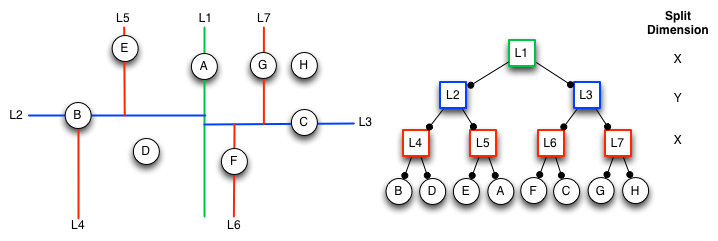
\includegraphics[width=0.9\textwidth]{rbffd_methods_content/neighbors/kdTree_example.png}
\caption{An example $k$-D Tree in 2-Dimensions. Nodes are partitioned with a cyclic dimension splitting rule (i.e., splits occur first in $X$, then $Y$, then $X$, etc.); all splits occur at the median node in each dimension. }
\label{fig:kdtree_example}
\end{figure}

Frequently, the terms \emph{$k$-D Tree} and \emph{Point $k$-D Tree} are used synonymously by the RBF community (see e.g., \cite{Fasshauer2007,FlyerLehto11,FornbergLehto11}); the same is convention adopted here. 

Generating an RBF-FD stencil with a $k$-D Tree can be efficiently accomplished in $O(n \log{N})$ time---where $n$ is the stencil size---following an approach introduced in \cite{Friedman1977}, and presented in Algorithm~\ref{alg:kdtree_knn}. The $k$-NN search starts a depth-first recursive search of the $k$-D Tree to find the nearest neighbor to a query point, $X_q$. Traversal of the the tree occurs by following branches left or right based on comparison of $X_q$ coordinates to the splitting value stored at each node of the tree, with the objective to find the smallest half-plane containing $X_q$. The search traverses the height of the tree in $O(\log N)$ steps to find the leaf that stores the nearest neighbor to $X_q$. The neighbor point and its distance from $X_q$ are inserted into a global priority queue, $pq$. Points in the priority queue are sorted in descending order according to distance. 


\begin{algorithm} 
\caption{KNNSearchKDTree($X_q$, $n$, $root$, $depth$)}         \label{alg:kdtree_knn}  
\begin{algorithmic}[1]    
    \State \textbf{Input:} A query node $X_q$, number of desired neighbors ($n$), the current \emph{root} of the $k$-D Tree, and the current $depth$ of traversal.
    \State \textbf{Output:} A global priority queue, $pq$, containing the $n$-nearest neighbors to $X_q$ sorted by distance from $X_q$ in descending order.
    \State \textbf{Assume:} A routine named ``BoundsOverlapBall" exists to determine if the boundaries of the current half-plane are intersected by the ball centered at $X_q$ with radius equal to the maximum distance in $pq$. As long as $pq.size < n$, ``BoundsOverlapBall" defaults to true. %$B_{+}$ and $B_{-}$ are $d$-dimensional arrays initialized to $\pm \infty$ on first call and used within BoundsOverlapBall.
    \State
    \If{$root$ is leaf}
        \State Insert $\{root,\text{dist}(X_q,root)\}$ into $pq$
        \If{$pq.\text{size} > n$} 
            \State $pq$.pop \Comment{Keep only $n$-nearest neighbors}
        \EndIf
        \State \Return
    \EndIf
    \State
    \If{$\text{coord}(X_q, depth) <= root.\text{value}$} 
       % \State $temp := B_{+}[depth]$, and $B_{+}[depth] := root.\text{value}$
        \State KNNSearchKDTree($X_q$, $n$, $root.\text{left}$, $(depth+1) \text{ \% } d$)
       % \State $B_{+}[depth] := temp$
    \Else
        %\State $temp := B_{-}[depth]$, and $B_{-}[depth] := root.\text{value}$
        \State KNNSearchKDTree($X_q$, $n$, $root.\text{right}$, $(depth+1) \text{ \% } d$)
       % \State $B_{-}[depth] := temp$
    \EndIf
    \State 
    \If{$\text{coord}(X_q, depth) <= root.\text{value}$} 
        %\State $temp := B_{-}[depth]$, and $B_{-}[depth] := root.\text{value}$
        \If{BoundsOverlapBall($X_q$)}
            \State KNNSearchKDTree($X_q$, $n$, $root.\text{right}$, $(depth+1) \text{ \% } d$)
        \EndIf
        %\State $B_{-}[depth] := temp$
    \Else
        %\State $temp := B_{-}[depth]$, and $B_{-}[depth] := root.\text{value}$
        \If{BoundsOverlapBall($X_q$)}
            \State KNNSearchKDTree($X_q$, $n$, $root.\text{left}$, $(depth+1) \text{ \% } d$)
        \EndIf
        %\State $B_{+}[depth] := temp$
    \EndIf
    \State \Return
    \end{algorithmic}
\end{algorithm}

After finding the nearest neighbor the algorithm returns to the previous split in the tree and traverses onto the opposing half-plane (i.e., down the far branch) to look for other leaves. So long as the size of $pq$ is at less than capacity ($n$) the search automatically adds points to the priority queue. If $pq$ reaches capacity the algorithm starts to pop off excess points with the understanding that the action removes those points farthest from $X_q$. 

In order to prune branches from the search and reduce complexity, Algorithm~\ref{alg:kdtree_knn} makes use of a routine called ``BoundsOverlapBall", which checks if any boundaries of the current level half-plane intersect/overlap with a closed ball centered at $X_q$. The ball is given a radius equal to the maximum distance in $pq$. Then, if the ball and a boundary intersect, the search will continue onto the half-plane on the opposite side of that boundary. This step handles the possibility that nearer nodes occur within the overlapped region in the other half-plane. If the ball and boundary do not intersect, the opposing half-plane and its related subtree are pruned from the search. Additional details on the implementation of ``BoundsOverlapBall" can be found in \cite{Friedman1977,TagliasacchiGC}. 

The authors of \cite{Friedman1977} find Algorithm~\ref{alg:kdtree_knn} capable of efficiently querying the $n$-nearest neighbors with a complexity proportional to $O(\log{N})$ (dominated by the cost of tree traversal). The relationship between stencil size $n$, and grid size, $N$, is better expressed as $O(n \log{N})$ for one stencil. 

RBF-FD only needs to generate stencils once, so the overall time for the step subsumes the cost of tree construction and $N$ queries. The resulting total complexity of stencil generation for all stencils is then proportional to $O(N\log{N})$. %The implementation of $k$-D Tree tested in Section~\ref{sec:stencils_benchmarks} reflects this complexity. 


% TODO: other related work. What implementations are available in MATLAB and C++?



\section{A Fixed-Grid Algorithm}

While a $k$-D Tree functions well for queries, the cost to build the tree structure is unnecessary overhead. Among the many data-structures that exist for nearest neighbor queries, alternatives like fixed-grid methods \cite{Samet2005,Wendland2002,WendlandBook} (a.k.a. uniform grid \cite{Krog2010,Green2010}) bypass much of the cost in construction with an assumption that only lower spatial dimensions (e.g., 2-D or 3-D) are significant for choosing neighbors. This discards the need to build a tree and shifts focus onto querying neighbors. 

Fixed-grid methods get their name from a coarse 2-D or 3-D regular grid that is overlaid on the domain. The $d$-dimensional grid divides the domain's axis aligned bounding box (AABB)---that is, the minimum bounding box containing the entire domain with edges parallel to axes---into $(h_n)^d$ cells. Subdivisions are uniform, so one can easily identify the cell containing any sample point, $p$, given the coordinates of the AABB and $(h_n)^d$. For example, let $(c_x, c_y, c_z)$ be the desired cell in 3-D, and $(x_{min}, y_{min}, z_{min})$ and $(x_{max}, y_{max}, z_{max})$ be the minimum and maximum coordinates of the AABB (resp.). Then the cell coordinates are found by:  
\begin{align}
(dx, dy, dz) & = \left(\frac{(x_{max} - x_{min})}{h_n}, \frac{(y_{max} - y_{min})}{h_n}, \frac{(z_{max} - z_{min})}{h_n}\right) \nonumber \\
(c_x, c_y, c_z) & = \left(\left\lfloor\frac{(p_x - x_{min})}{dx}\right\rfloor , \left\lfloor\frac{(p_y - y_{min})}{dy}\right\rfloor , \left\lfloor\frac{(p_z - z_{min})}{dz}\right\rfloor \right).
\label{eq:cell_hash}
\end{align}
Cells neighboring $(c_x, c_y, c_z)$ are trivial to find by adding positive and negative offsets to each coordinate. %Note that the fixed-grid in this method is virtual. Nodes are matched with cell coordinates, but the full grid (i.e., vertices/edges) is never explicitly constructed.

Fixed grid methods also make use of \emph{space filling curves}. Space filling curves pass through every point in $d$-dimensional space, and through each point only once. Equivalently, space filling curves map $d$-dimensional space down to 1-D, where every point is converted to a unique index or traversal order based on its spatial coordinates. These mapping properties make space filling curves ideal for use as hash functions. Traversing the $d$-dimensional points (i.e., playing ``connect the dots") draws the space filling curve. Figure~\ref{fig:space_filling_curves} presents two common orderings of a 2-D fixed-grid. Note that one-dimensional orderings are not unique. On the left is a \emph{Raster}-ordering (a.k.a. Scanline- or $ijk$-ordering): $f(c_x,c_y,c_z) = ((c_x * h_n) + c_y) * h_n + c_z$. The right half of Figure~\ref{fig:space_filling_curves} shows an ordering known as Morton- or $Z$-ordering. $Z$-ordering construction is discussed later in this chapter. On both sides of Figure~\ref{fig:space_filling_curves}, the lower left corner of each cell indicates the mapped index. Traversing the cells in order produces the curves superimposed in red. 

\begin{figure}
\centering
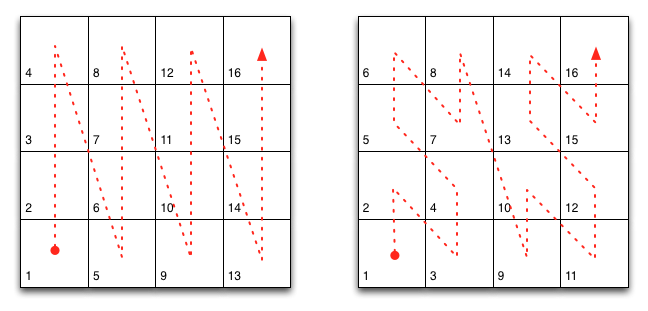
\includegraphics[width=0.65\textwidth]{rbffd_methods_content/neighbors/space_filling_curves.png}
\caption{Two example space filling curves to linearize the same fixed-grid. Left: Raster-ordering ($ijk$); Right: Morton-/Z-ordering.}
\label{fig:space_filling_curves}
\end{figure} 


At a high level, fixed-grid methods have the following construction steps \cite{Krog2010}:
\begin{enumerate}
\item Subdivide the domain with the overlay grid.
\item For each node, identify the containing cell coordinates.
\item For each node, use the cell coordinates as input to a spatial hash function (i.e., a space-filling curve).
\item Sort the nodes according to their spatial hash.
\end{enumerate}
Particular details of how nodes are sorted, the choice of hashing function, the number of nodes allowed per cell, etc. determine the specific class of fixed-grid method and corresponding complexity. A comprehensive list of options and classifications can be found in \cite{Samet2005}. 

\subsection{Fixed-grid Construction}
The algorithm in this work is inspired by fixed-grid approaches for GPU particle simulations (\cite{Krog2010,Green2010,Johnson2011}). Particle methods require a ball query at each time-step. With time-steps often dominated by the cost of querying neighbors, the community understandably devotes significant effort to seek out the most efficient solutions possible \cite{Goswami2010}. The fixed-grid method is competitive for at least two reasons: a) by bypassing the need to build a tree, half the cost in querying neighbors is avoided; and b) nodes sorted according to a spatial hash reside closer in memory to nearby neighbors than in the case of unsorted nodes. The spatial locality results in a higher likelihood that data will be cached when required. Note that reordering by cell hash sorts nodes across cells but not within them---that is, nodes contained by the same cell are contiguous in memory, but remain arbitrarily ordered with respect one another. Fortunately, with contiguous groups of nodes, nearest neighbor queries can directly access all nodes per cell. 


The authors of \cite{Krog2010,Johnson2011,Green2010} assume a raster-ordering on cells, and that the uniform grid is sufficiently refined to ensure cells contain at most eight nodes. Particle interactions are limited to ball queries on the containing cell plus one valence of neighboring cells (i.e., 8 surrounding cells in 2-D and 26 cells in 3-D). Since the number of cells to check is fixed, the neighboring nodes can be obtained by direct access in constant time. A similar approach is taken by \cite{Goswami2010}, but the authors opt for a $Z$-ordering of cells. 
 As a point of difference in implementations, the authors of \cite{Green2010, Krog2010, Goswami2010} leverage a fast radix sort algorithm to order nodes based on hash index, while \cite{Johnson2011} utilizes a slower bitonic sort algorithm. The fixed-grid in \cite{Wendland2002,WendlandBook} forgoes logic to refine the grid and enforce a maximum limit on the number of nodes per cell. The author also avoids sorting nodes based on cell hashes. Instead, a list is maintained that stores the indices of all contained nodes per cell. %, which implies random memory access when operating on the nodes of a cell.    


The implementation presented here is a hybrid of the related algorithms. For example, cells are sorted based on raster-ordering, but without the restriction on max number of nodes per cell. Rather than a radix- or bitonic sort to reorder nodes, the list of node indices for each cell (\cite{Wendland2002,WendlandBook}) is constructed as part of a single-pass bucket sort. Finally, in stark contrast to  \cite{Krog2010,Green2010,Johnson2011,Wendland2002,WendlandBook}, querying neighbors is not restricted to a fixed radius, or number of cell valences. To satisfy the $k$-NN query, this implementation iteratively increases the query radius to include a new valence of cells at each iteration. This multi-pass ball-query was demonstrated in Figure~\ref{fig:nearest_neighbor_example}. The iteration terminates when the desired count of neighboring nodes is satisfied or exceeded.
%TODO: Figure~\ref{fig:hash_highlevel} demonstrates the algorithm 
%\begin{figure}
%\centering
%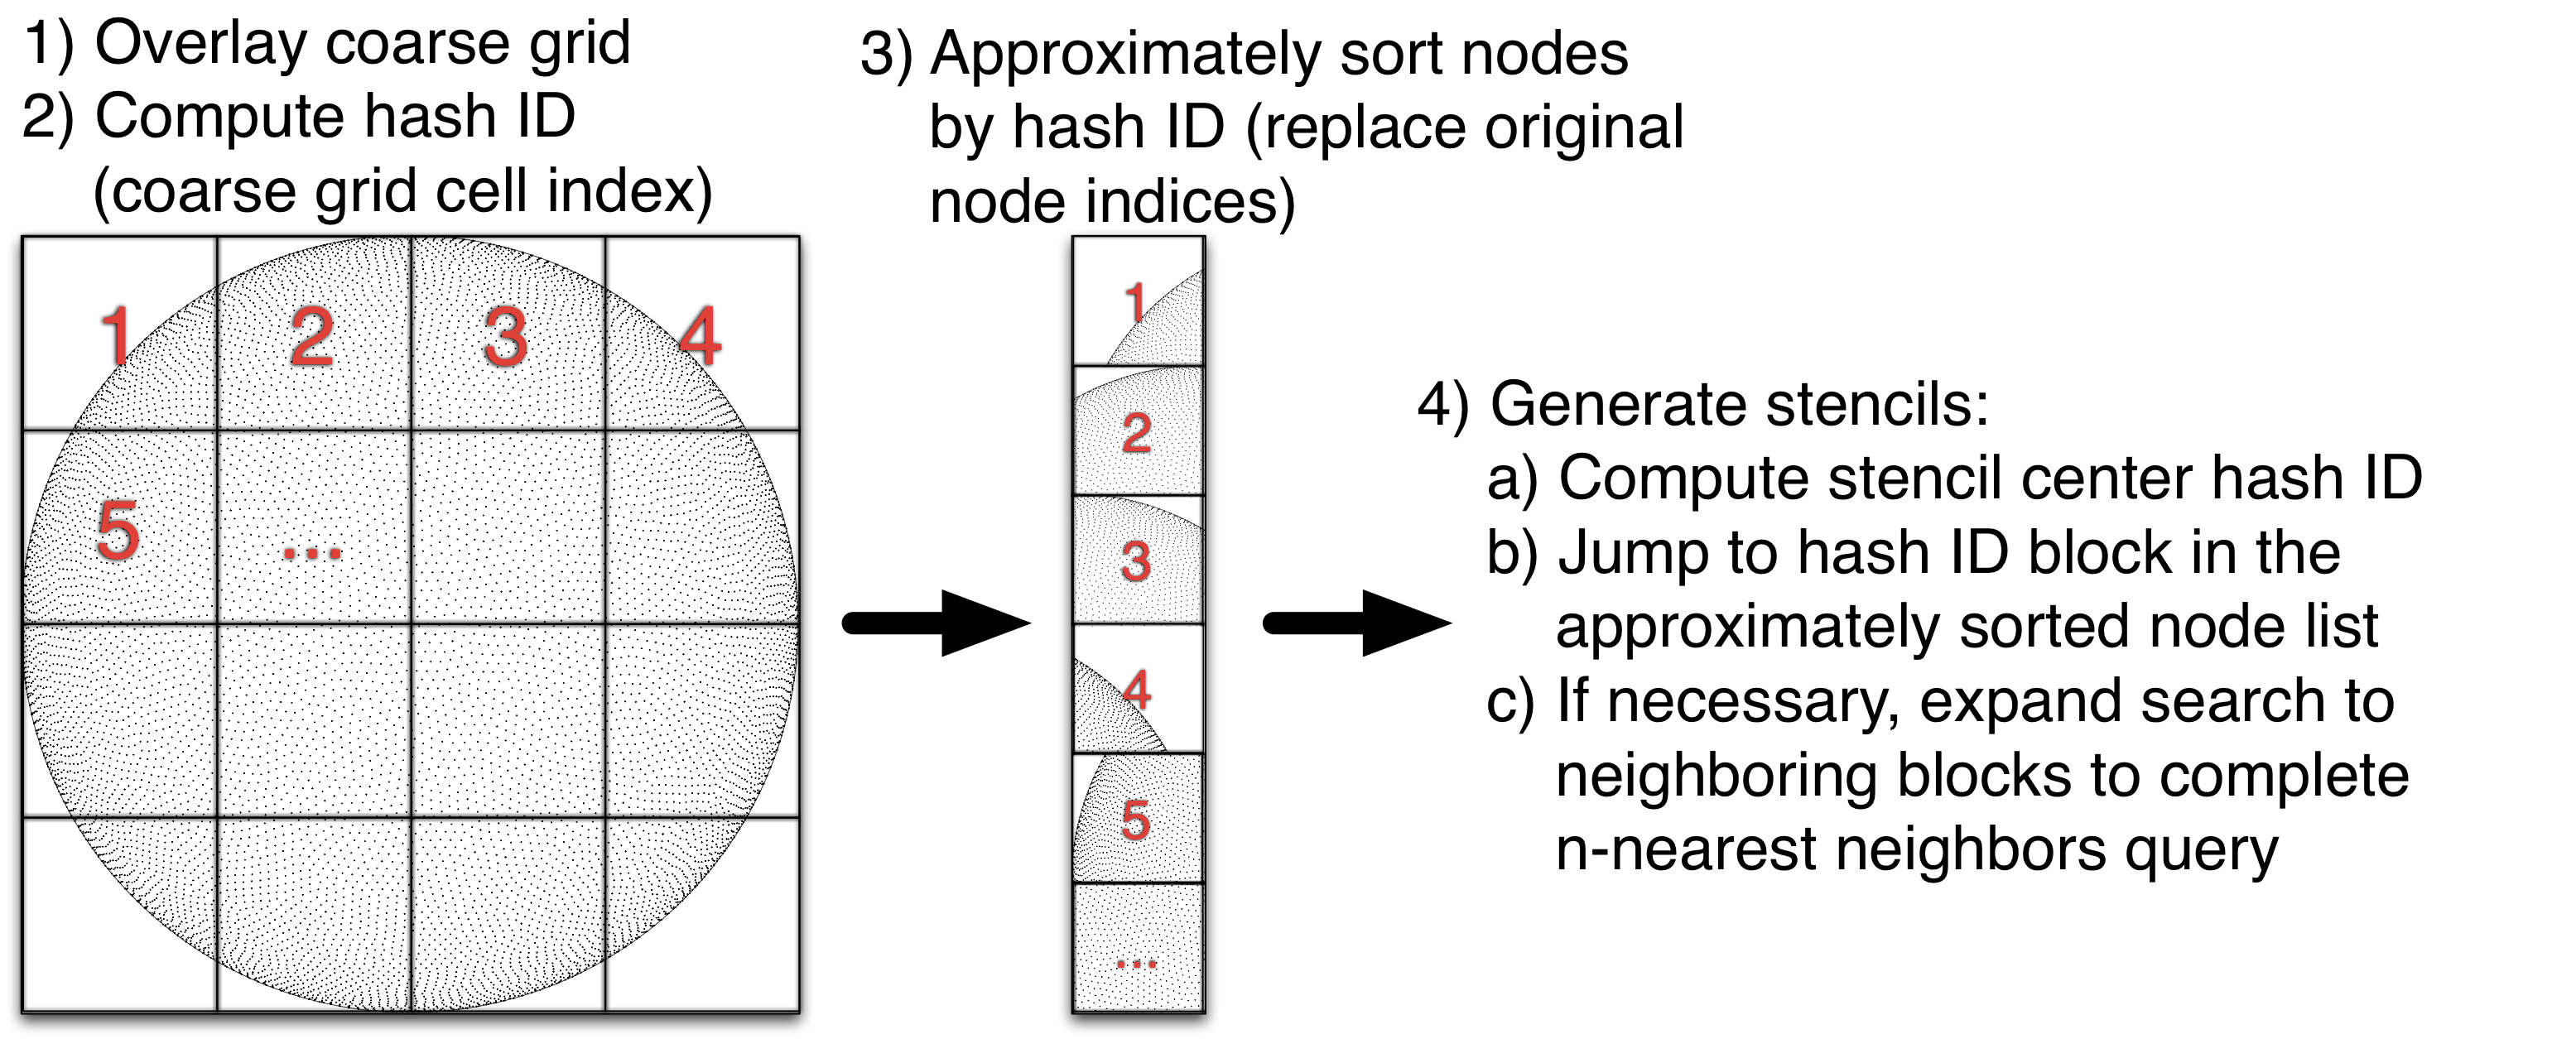
\includegraphics[width=1.0\textwidth]{../figures/chapter2/hashing_example/LSH_Concept.png}
%\caption{High level overview of the \emph{Fixed-Grid Bucket} (a.k.a. Hash) Algorithm. A coarse regular grid is overlaid on the domain. Nodes coordinates are hashed to containing cell indices and pushed onto a list for the appropriate cell. The cells are reordered in memory according to a space filling curve (i.e., Raster (IJK), Morton (Z), Graycode (U), etc.). Stencil queries start search with the cell containing the stencil center and expand to neighboring cells until at least $n$ candidate nodes are found. The candidate list is truncated to the $n$ closest neighbors. }
%\label{fig:hash_highlevel}
%\end{figure} 

\begin{algorithm} 
\caption{BuildFixedGrid($P$, $h_n$)}         
\label{alg:fixed_grid_build}  
\begin{algorithmic}[1]    
    \State \textbf{Input:} A set points $P$, and the fixed-grid resolution, $h_n$.
    \State \textbf{Output:} The reordered points in $P$, and corresponding cell buckets $Q$.
    \State
    \State Create $Q$: an $(h_n)^d$ array of empty buckets. 
    \For{point $p_i$ in $P$}
       \State $c := \text{CellCoords}(p_i)$ 
       \State $ind := \text{SpatialHash}(c)$
       \State Append index $i$ onto $Q[ind]$
    \EndFor
    \For{$j=0,1,...,(h_n)^d$}
    \If{$Q[j]$ is not empty}
        \State Append the set $P[Q[j]]$ onto $\hat{P}$
        \State Overwrite the set $Q[j]$ with new indices of $\hat{P}$ 
    \EndIf
    \EndFor
    \State $P := \hat{P}$
    \State \Return 
    \end{algorithmic}
\end{algorithm}

Algorithm~\ref{alg:fixed_grid_build} presents the fixed-grid build process. The routine starts with the allocation an array of empty buckets, $Q$. Next $Q$ is populated based on the spatially hashed cell coordinates. The second for-loop in Algorithm~\ref{alg:fixed_grid_build} iterates through $Q$, looking for non-empty buckets. When one is found, nodes referenced by that bucket are transcribed/appended onto the ``sorted" list of nodes $\hat{P}$. This way the nodes in each cell are contiguous, but maintain the original ordering with respect to one another. Additionally, node indices in $\hat{P}$ replace the old indices within $Q$.

The entire build process complexity is proportional to $O(N)$, and requires $O((h_n)^d + N)$ storage. Samet \cite{Samet2005} would classify this approach as a \emph{fixed-grid bucket method with one-dimensional ordering}. The term \emph{bucket} refers to the allowance for each cell to contain an arbitrary number of nodes. \emph{One-dimensional ordering} is indicative of attempts later in the chapter to employ alternative space-filling curves in place of raster-ordering. 

A special note: the final step of Algorithm~\ref{alg:fixed_grid_build} overwrites the original list of nodes with the sorted equivalent. The spatially sorted list is included in the cost of stencil generation, but available for reuse elsewhere. Since the first step in RBF-FD applications is to generate stencils, overwriting the input node set can guarantee that the node values throughout the entire life-cycle of an RBF-FD application will benefit from the same spatial locality as stencil generation. This benefit is (almost) free. 

Consider Figure~\ref{fig:reorder_example}, which shows two differentiation matrices generated based on the same $N=6400$ MD-node set (unit sphere), with each row representing an RBF-FD stencil of $n=50$ non-zeros. The left matrix in Figure~\ref{fig:reorder_example} is generated with stencils queried by a $k$-D Tree. The $k$-D Tree maintains the original ordering on $P$. The matrix on the right of Figure~\ref{fig:reorder_example} is a permuted equivalent of the left matrix with fixed-grid cells sorted based on a raster-ordering for $h_n = 10$. 

Looking at Figure~\ref{fig:reorder_example} it should be obvious that reordering the nodes can improve memory access patterns for SpMV. If each row is applied as a sparse dot-product with a dense vector, the more condensed non-zeros are in the row, the more likely values from the dense vector will be resident in cache when needed. Likewise, non-zeros that appear on consecutive rows can benefit from cache reuse. Later in this chapter, the impact of spatial orderings are compared to determine how RBF-FD can benefit the most. 

\begin{figure}
\centering
\begin{subfigure}{0.425\textwidth}
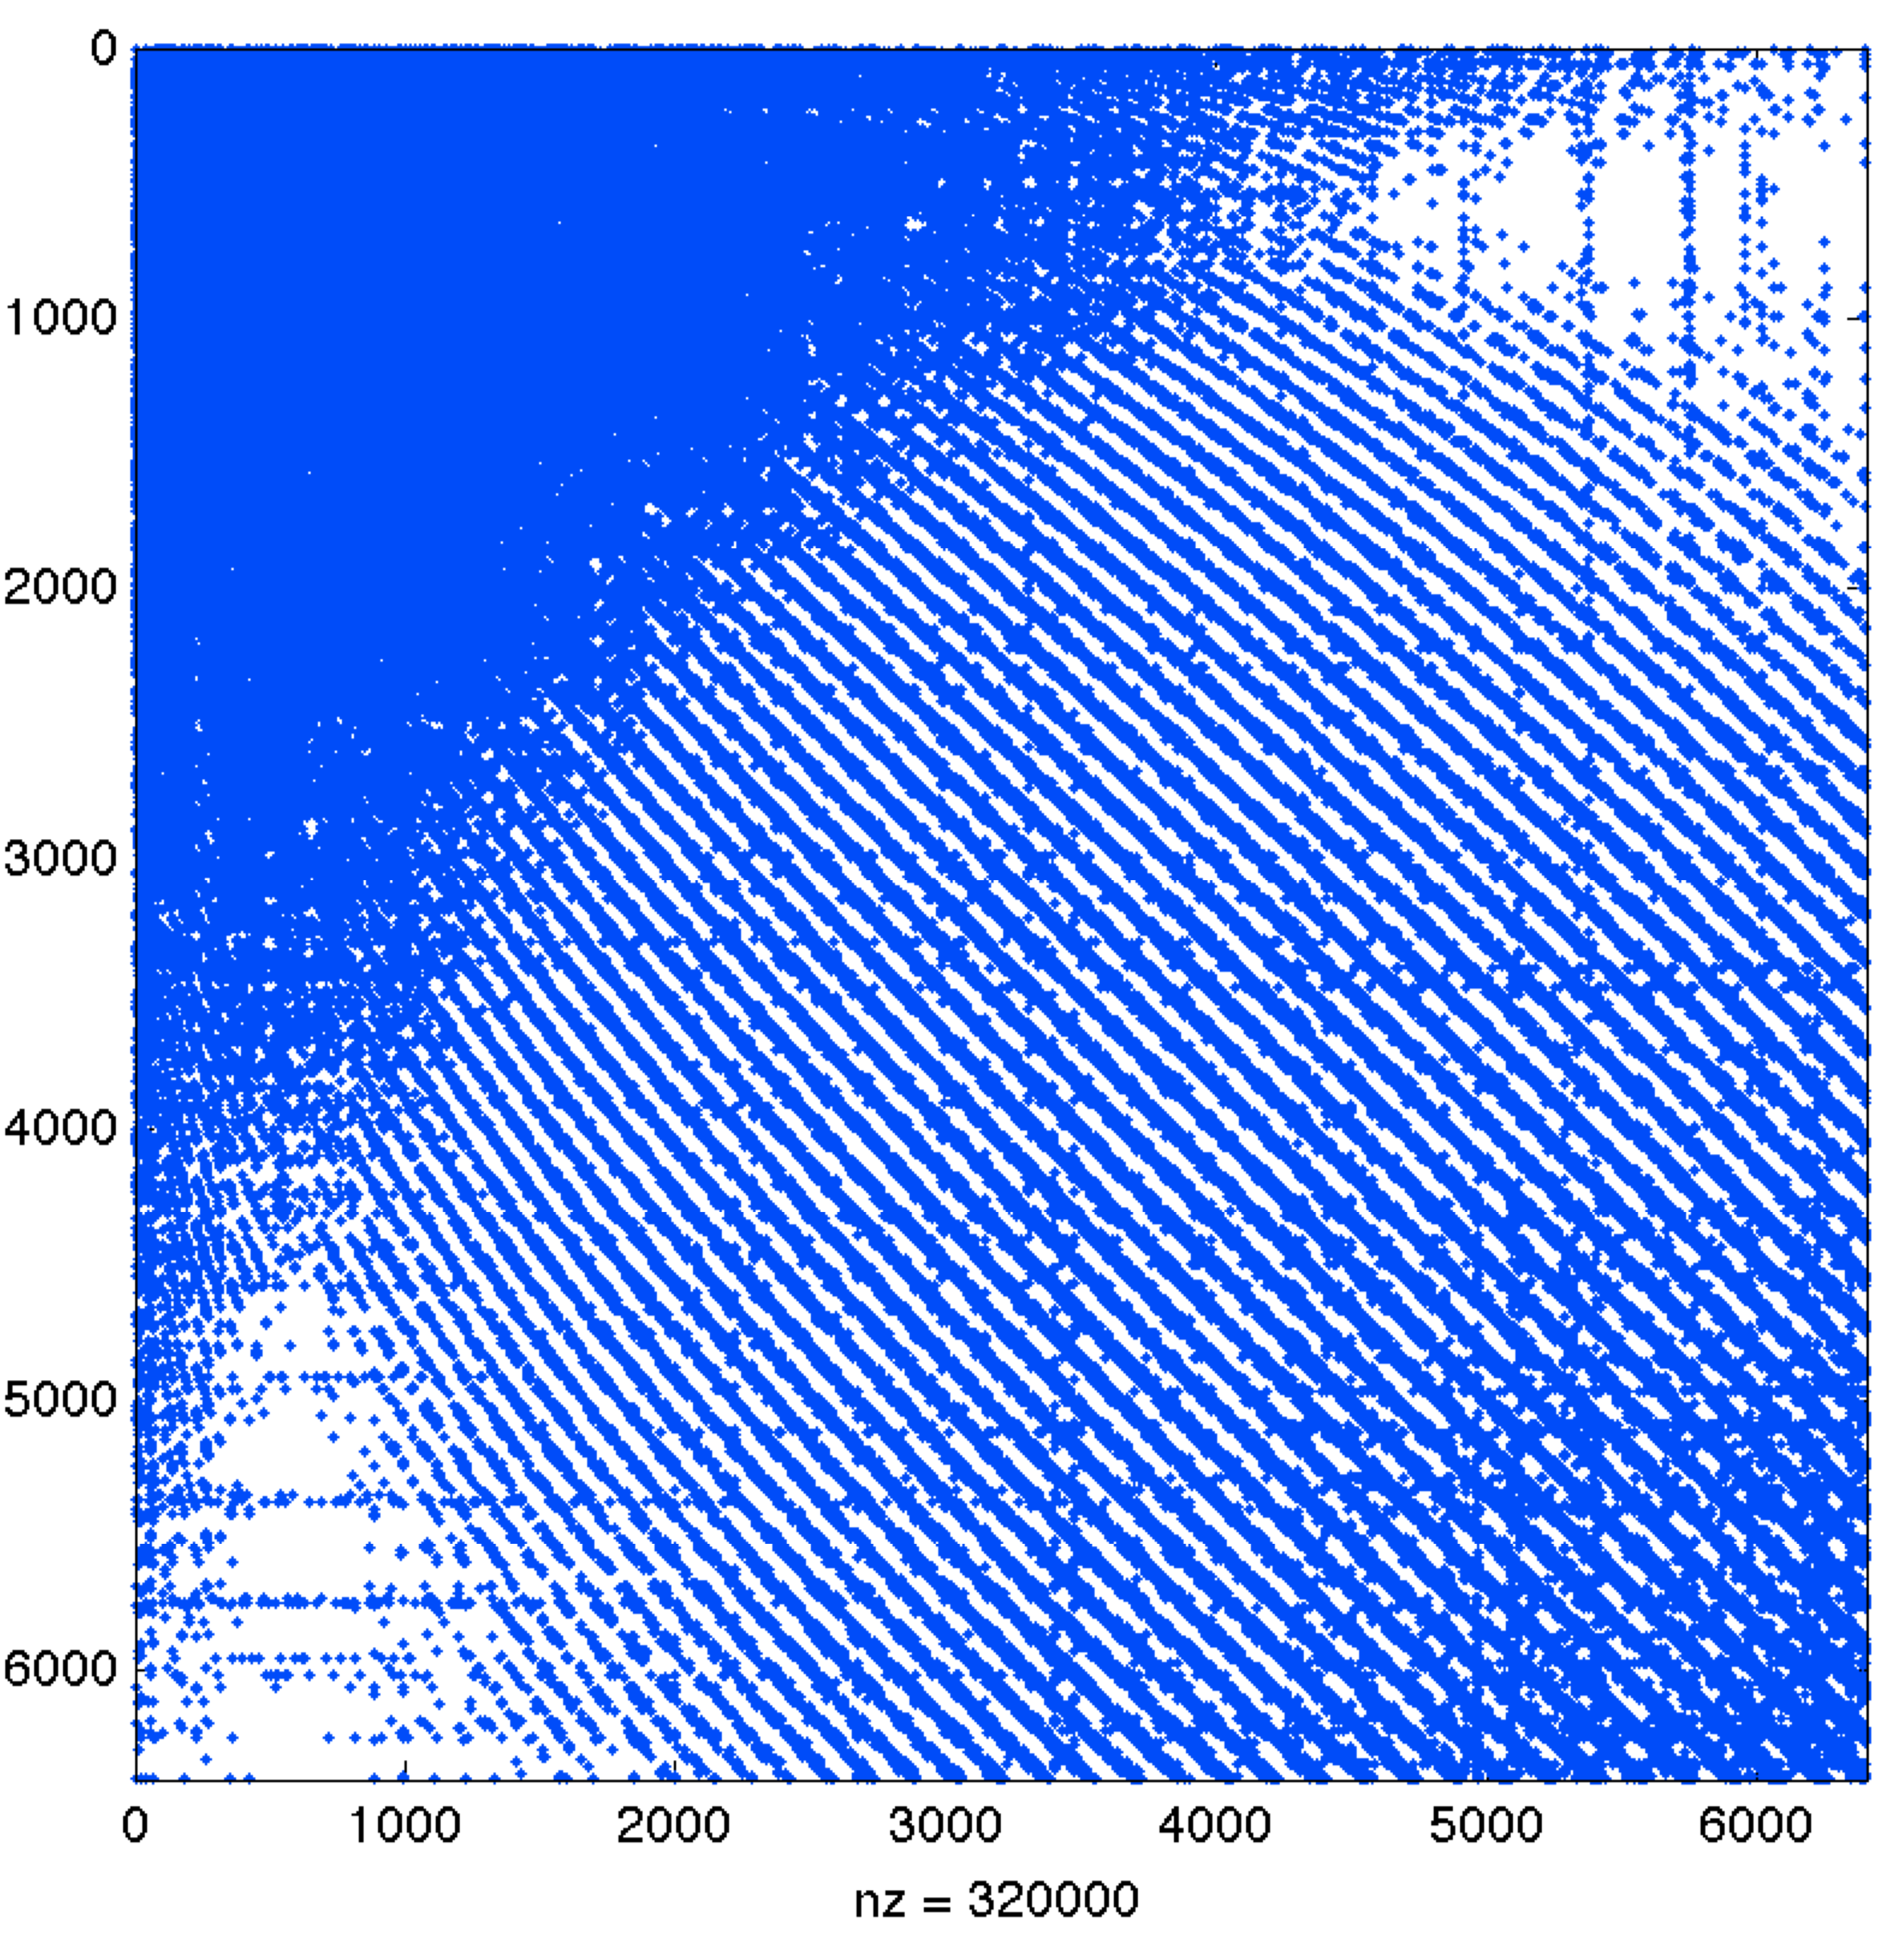
\includegraphics[width=1.0\textwidth]{../figures/chapter2/hashing_example/bruteforce_N6400_n50-eps-converted-to.png}
\caption{$k$-D Tree} 
\end{subfigure} 
\begin{subfigure}{0.425\textwidth}
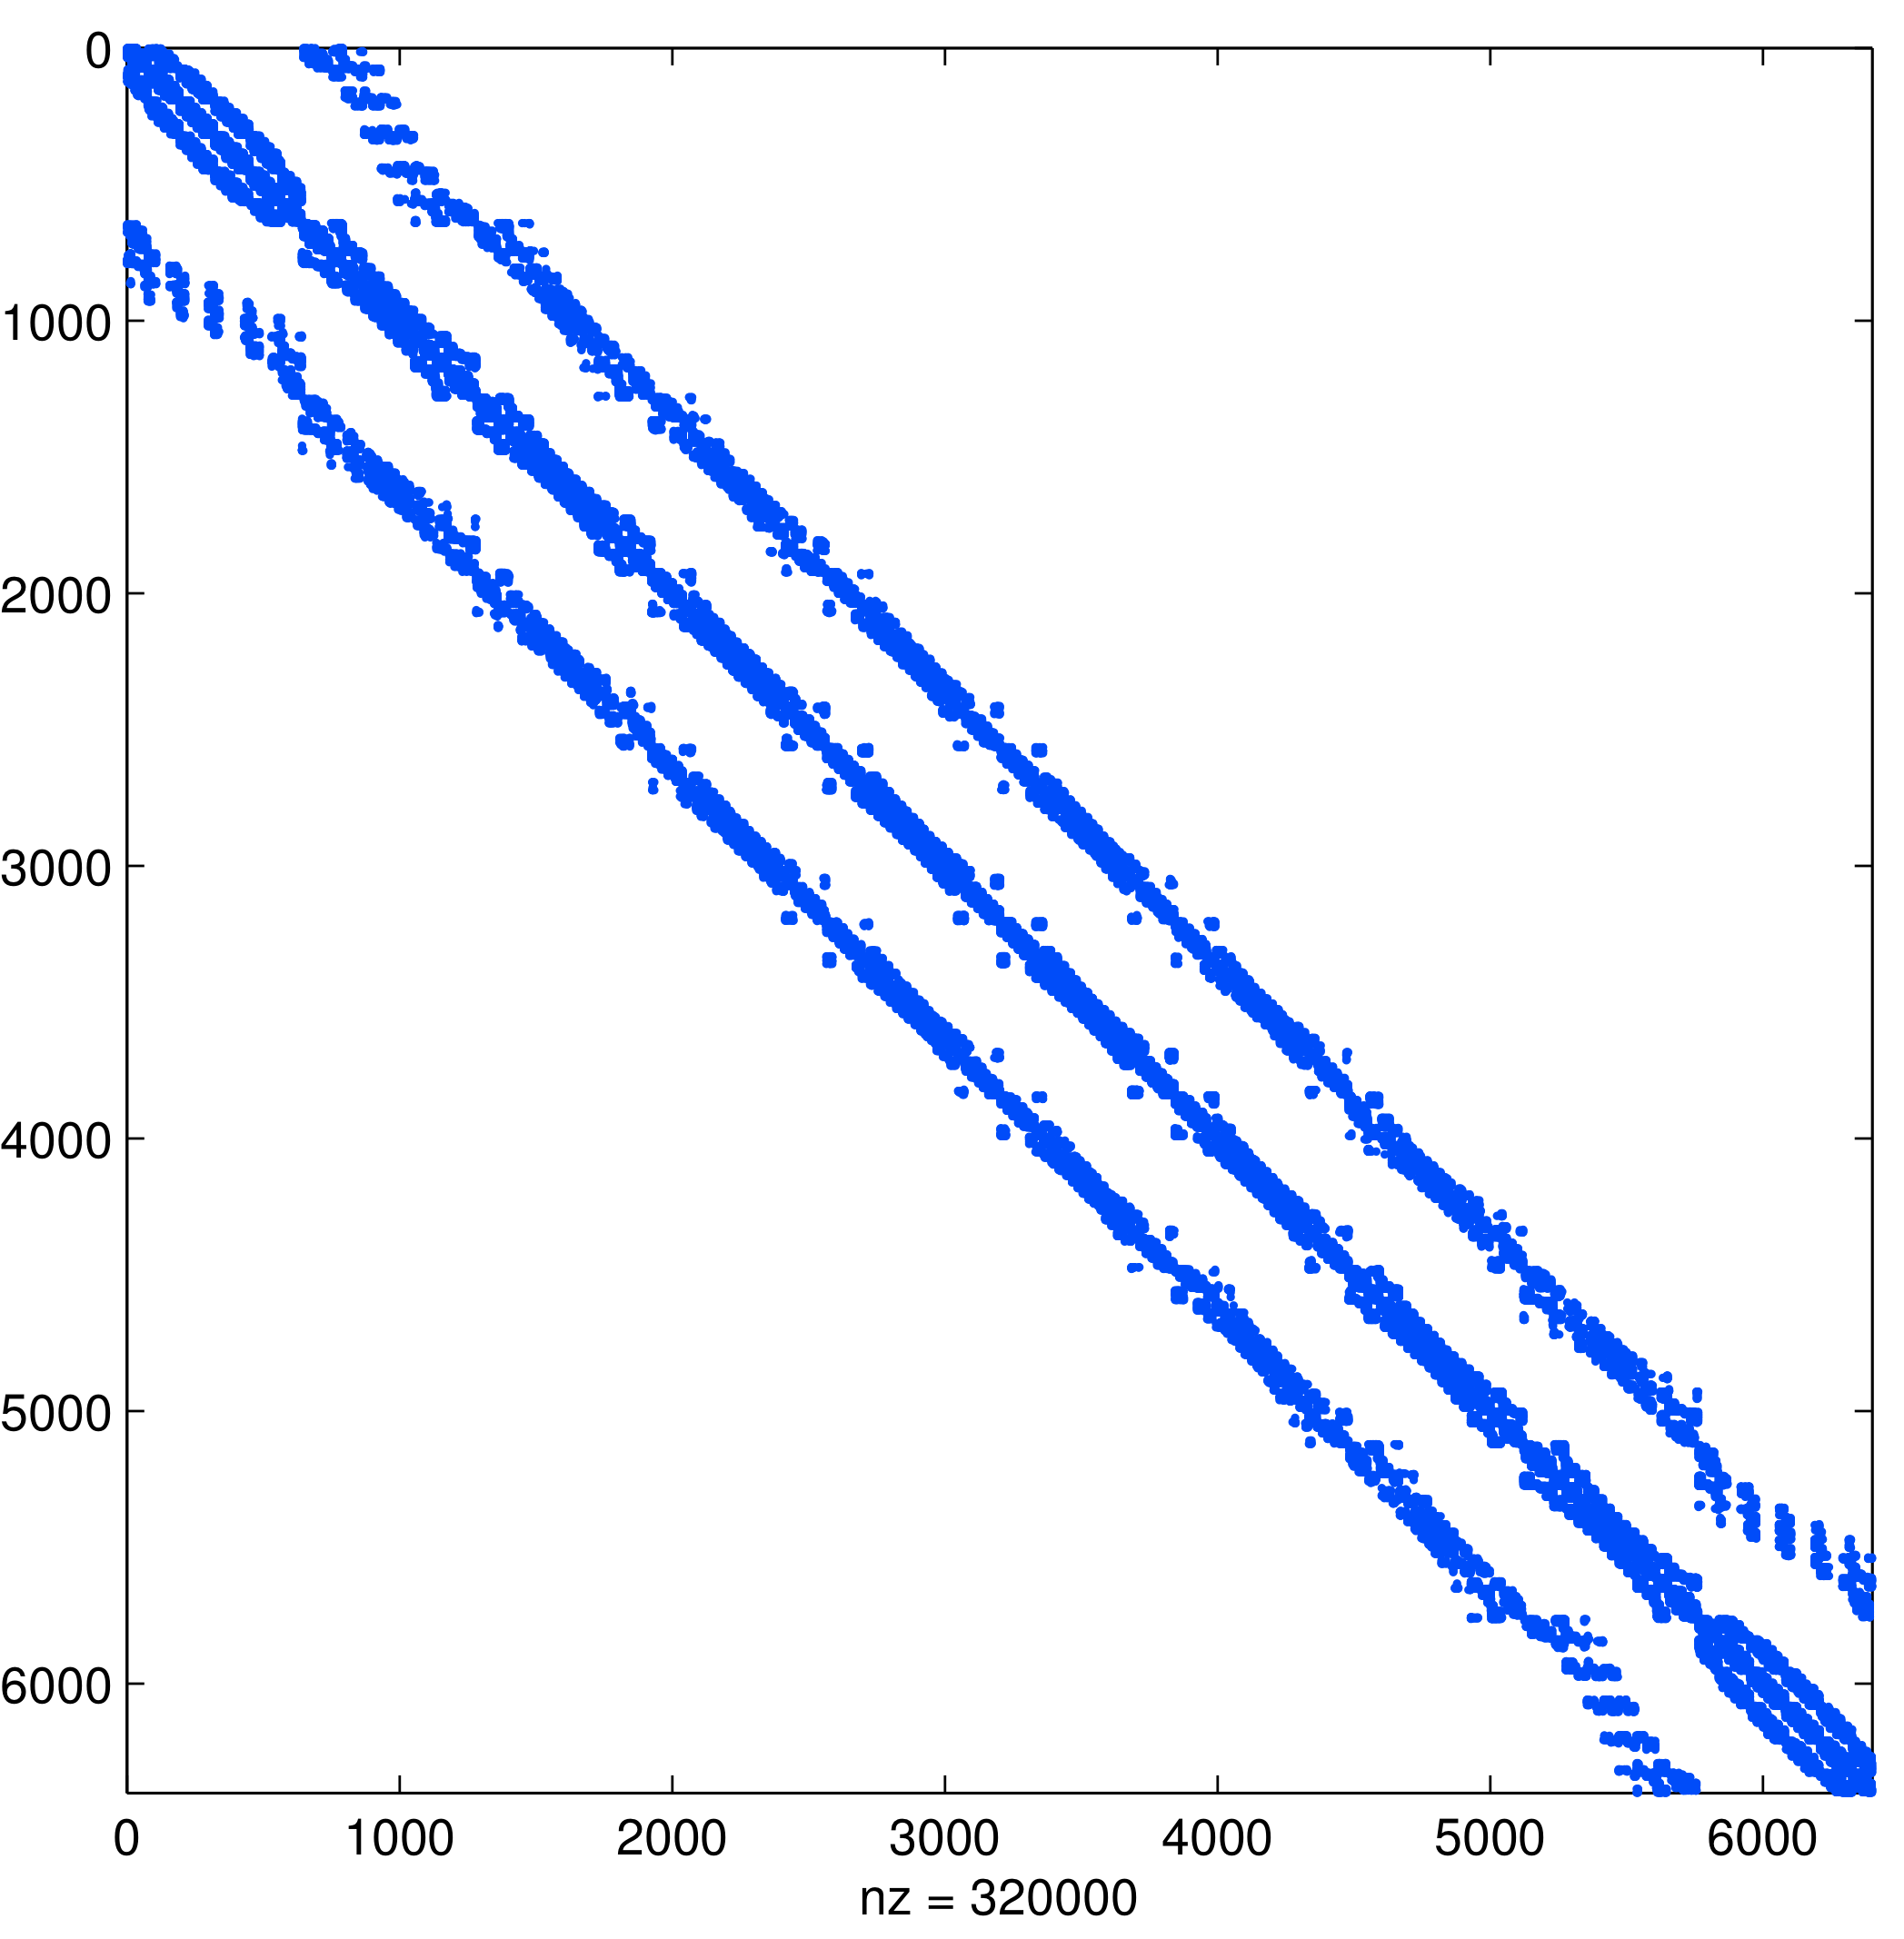
\includegraphics[width=1.0\textwidth]{../figures/chapter2/hashing_example/lsh_N6400_n50-eps-converted-to.png}
\caption{Fixed-Grid}
\end{subfigure}
\caption{Example effects of node reordering for MD node set $N=6400$ with $n=50$. The differentiation matrices are permuted equivalents and roughly $0.78\%$ full. a) Stencils generated based on $k$-D Tree maintain the original node ordering. b) The reordered node set generated using an $h_n=10$ fixed-grid condenses non-zeros for improved memory access patterns (i.e., cache reuse).}
\label{fig:reorder_example}
\end{figure} 

\subsection{Fixed-Grid Neighbor Query}

Querying the $k$-nearest neighbors for a single query node, $X_q$, is the subject of Algorithm~\ref{alg:fixed_grid_query}. The process begins by finding $X_q$'s containing cell, $c$. The hash value of $c$ is used to identify (in $Q$) the list of nodes contained within that cell, all of which are appended to a vector of neighbor candidates, $pq$. 

It is possible for the number nodes in $c$ to exceed $n$; however, the algorithm conservatively assumes that it is necessary to search at least one valence of cells around it.  This ensures that nodes near the cell boundaries will find nearby neighbors outside of $c$, and the stencils will balanced. For certain fixed-grid resolutions, a single valence may not satisfy the stencil size requirements, so the algorithm iterates outward onto new valences. As cells are checked, their nodes are appended onto $pq$. 

The final stage of Algorithm~\ref{alg:fixed_grid_query} calculates the distance from all candidate nodes to $X_q$, and uses that metric to sort $pq$ in ascending order. The first $n$ nodes in $pq$ are returned as the stencil. 
\begin{algorithm} 
\caption{QueryFixedGrid($X_q$, $n$, $P$, $Q$ )}         
\label{alg:fixed_grid_query}  
\begin{algorithmic}[1]    
    \State \textbf{Input:} A query point, $X_q$; the desired number of neighbors, $n$; a set of $d$-dimensional points $P$; and the matching cell bucket list, $Q$.
    \State \textbf{Output:} The $n$-nearest neighbors list $pq$.
    \State     
    \State $valence := 1$
    \State $c := \text{CellCoords}(X_q)$ 
    \State $ind := \text{SpatialHash}(cells)$
    \State Append $P[Q[ind]]$ onto $pq$
    \While{$pq$.size $< n$ OR $valence < 2$}
        \State $cells := \text{NeighboringCellCoords}(c, valence)$
        \State $inds := \text{SpatialHash}(cells)$
        \For{each $q$ in $Q[inds]$}
            \If{$q$ is not empty} 
            \State Append node list $P[q]$ onto $pq$
            \EndIf
        \EndFor
        \State increment $valence$
    \EndWhile
    \State $dists := \text{ComputeDistances}(pq)$
    \State Sort $pq$ by $dists$
    \State \Return the first $n$ nodes in $pq$
    \end{algorithmic}
\end{algorithm}


Complexity of Algorithm~\ref{alg:fixed_grid_query} can vary based on the choice of $h_n$. For a sufficiently refined fixed-grid the $k$-ANN is dominated by the cost of the \emph{while-loop} and behaves as $O(\log h_n)$ per stencil. In the worst case, when $h_n$ is small, the cost of sorting $pq$ dominates, and is proportional to $O(N \log N)$ (using a C++ STL Sort) in the worst case. %TODO: verify with Gordon.  
Results below demonstrate that proper choice of $h_n$ can maintain logarithmic complexity similar to the $k$-D Tree query. 


The fixed grid query algorithm is considered an \emph{approximate nearest neighbor} (ANN) search. Consider again the nodes in Figure~\ref{fig:nearest_neighbor_example}. A $k$-NN stencil of size $n=8$ should contain the green center, all blue nodes, plus the red node and one black node. The true $k$-NN would select the black node in the right-most column of the grid (i.e. the node closer to the dashed ball query). Under the fixed-grid method, however, the alternative black node is selected even though it is more distant. This is true because the more distant black node occupies the second valence of cells around the stencil center, whereas the true near neighbor is in the third valence. Algorithm~\ref{alg:fixed_grid_query} is able to truncate the search in the second valence by satisfying the requirement on $n$. 

Similarly, if cells were rectangular in shape, the ball-query would end up an ellipsoid and stencils would be biased with more nodes in one direction. To combat this, and ensure spherical stencils, this work assumes the AABB bounding the domain is a cube (i.e., $dx = dy = dz$). 

The difference between a true $k$-NN and $k$-ANN is insignificant from the perspective of RBF-FD. The method compensates automatically for differences in node locations when weights are calculated. On top of this, the only differences in stencils generated by $k$-NN versus $k$-ANN occur at nodes on the outermost reaches of the stencil (i.e., nodes with the least impact on the stencil center).


%\begin{figure}
%\centering
%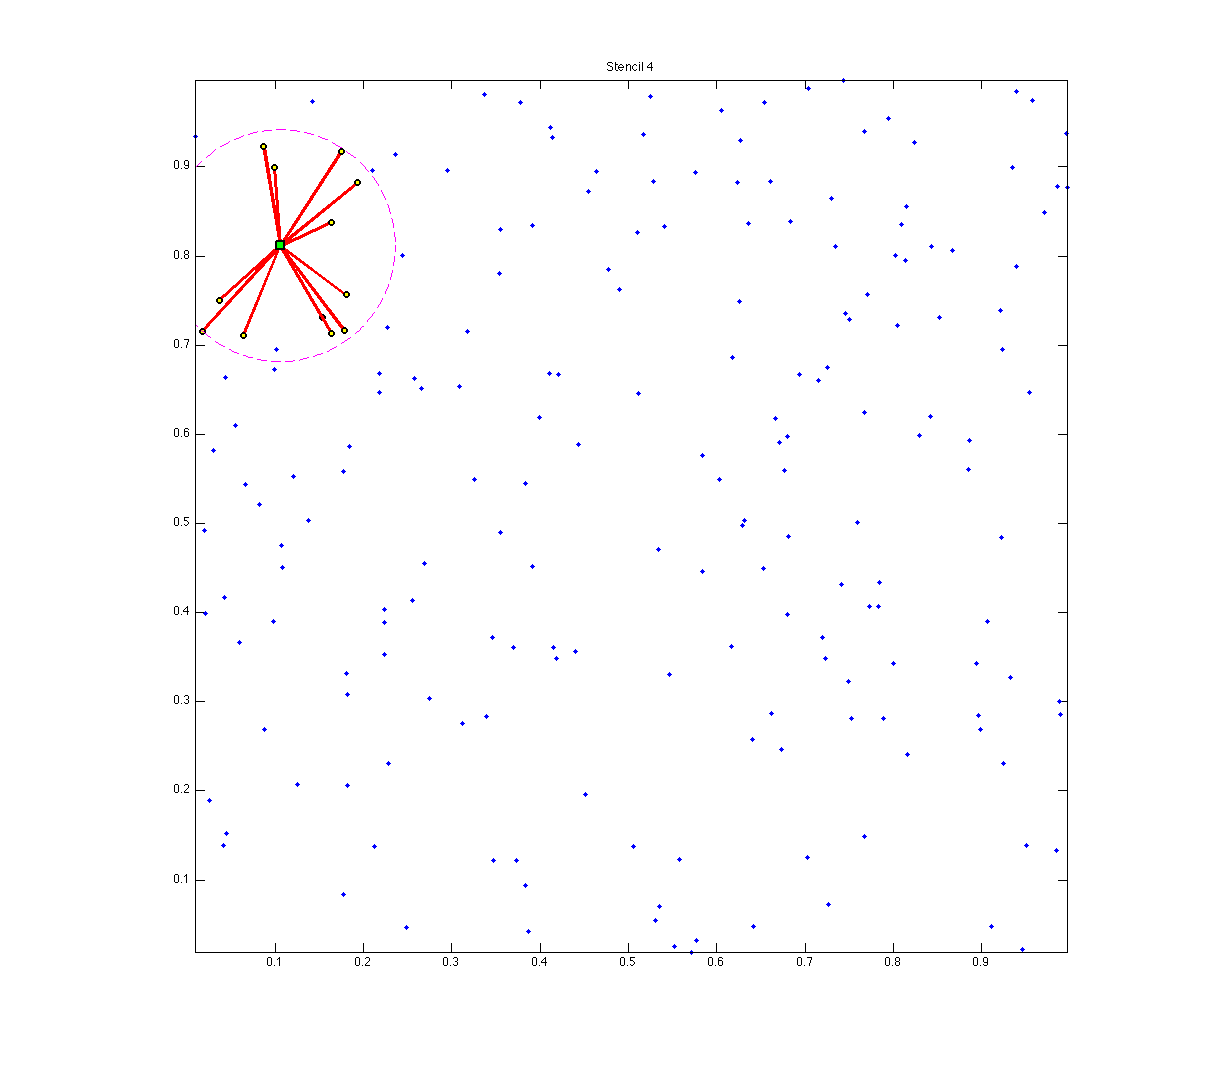
\includegraphics[width=8.5cm]{rbffd_methods_content/neighbors/neighbor_incorrect.png}
%\caption{A stencil generated with $k$-ANN satisfies the required stencil size, but is not guaranteed to choose the true nearest neighbors.}
%\label{fig:approximate_nearest_neighbors}
%\end{figure}

\subsection{Performance Comparison}

This implementation is CPU only. Porting the one time stencil generation to the GPU was seen as 


The $k$-D tree implementation compared in this work is the \emph{$kd$-Tree Matlab} library from Tagliasacchi \cite{TagliasacchiMFE,TagliasacchiGC}. Originally posted to the Matlab FileExchange and now maintained as a Google Code project. Until the addition of $KNNsearcher$ in Matlab 

garnered attention due to its MEX compiled interface that allowed use as both a C++ and MATLAB library. 
The Matlab central $k$-D Tree is MEX compiled and efficient. We integrated the standalone C++ code into our library.  

Tagliasacchi \cite{TagliasacchiGC} follows the algorithms preneted above and uses the standard split by median in each dimension, with alternating chosen by incrementing the dimension by one, modulo the number of dimensions (e.g., in 2D the order is $X, Y, X, Y, ...$). Wendland \cite{WendlandBook} suggests a number of more advanced median cuts such as 

\cite{TagliasacchiMFE}. 
\cite{MatlabKDTreeSearcher}



what is best overlay resolution? based on time to generate. choose resolution as n/2, n/9? etc? 




At the onset of our work on RBF-FD, the most commonly used KDTree implmentation used by the RBF community was \cite{Tagliasacchi2008}. Recently, improvements were made to the KDTree algorithm to reduce the cost of building the KDTree to $O(N log^2 N)$. 

Figure~\ref{fig:stencil_query_old_and_new} compares the total time to generate $N$ stencils of size $n=50$ with three methods: \cite{Tagliasacchi2008}, our hash-based neighbor query, and the improved KDTree from \cite{Tagliasacchi2012}. 
Until the new release of KDTree, our algorithm was a major improvement to the performance of stencil generation. The hash-based approach achieved greater than 







\begin{figure}
\centering
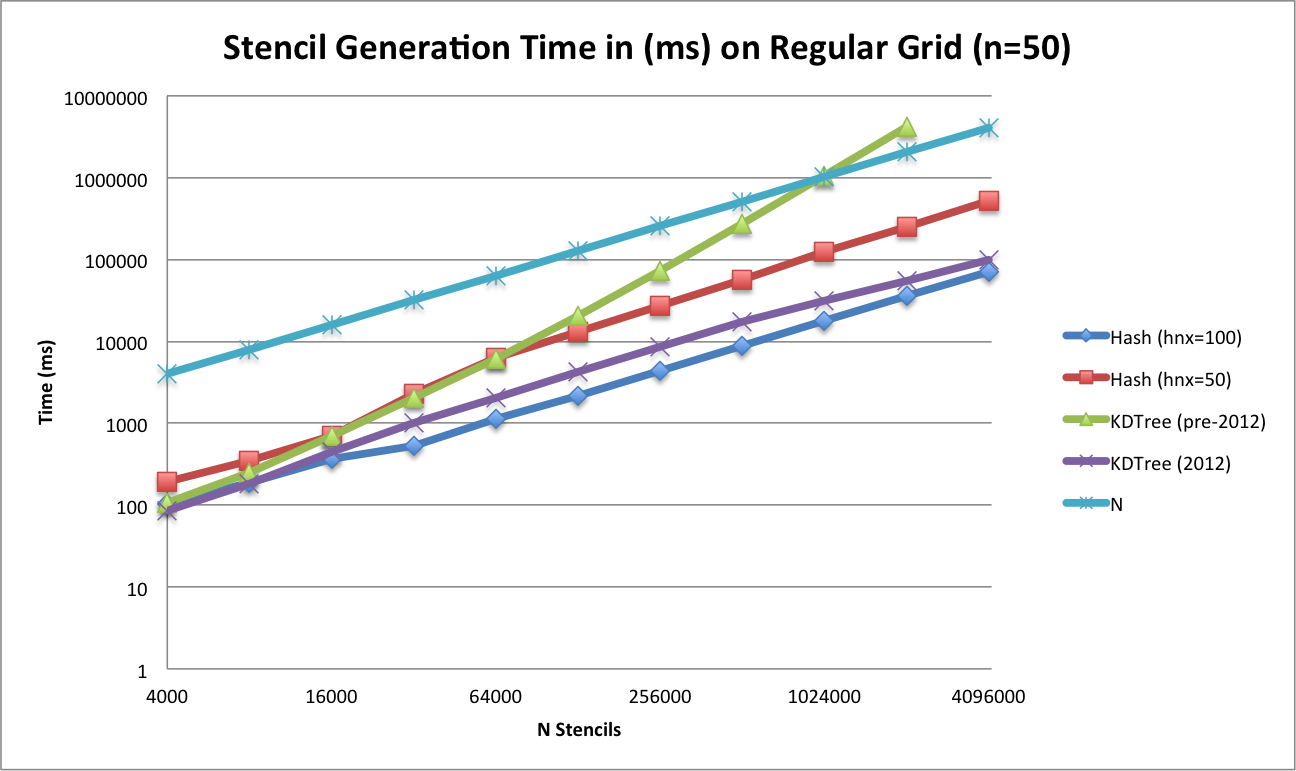
\includegraphics[width=9.5cm]{../figures/stencils/kdtree_old_reg_subsets_4m_stencil_gen_time.png}
%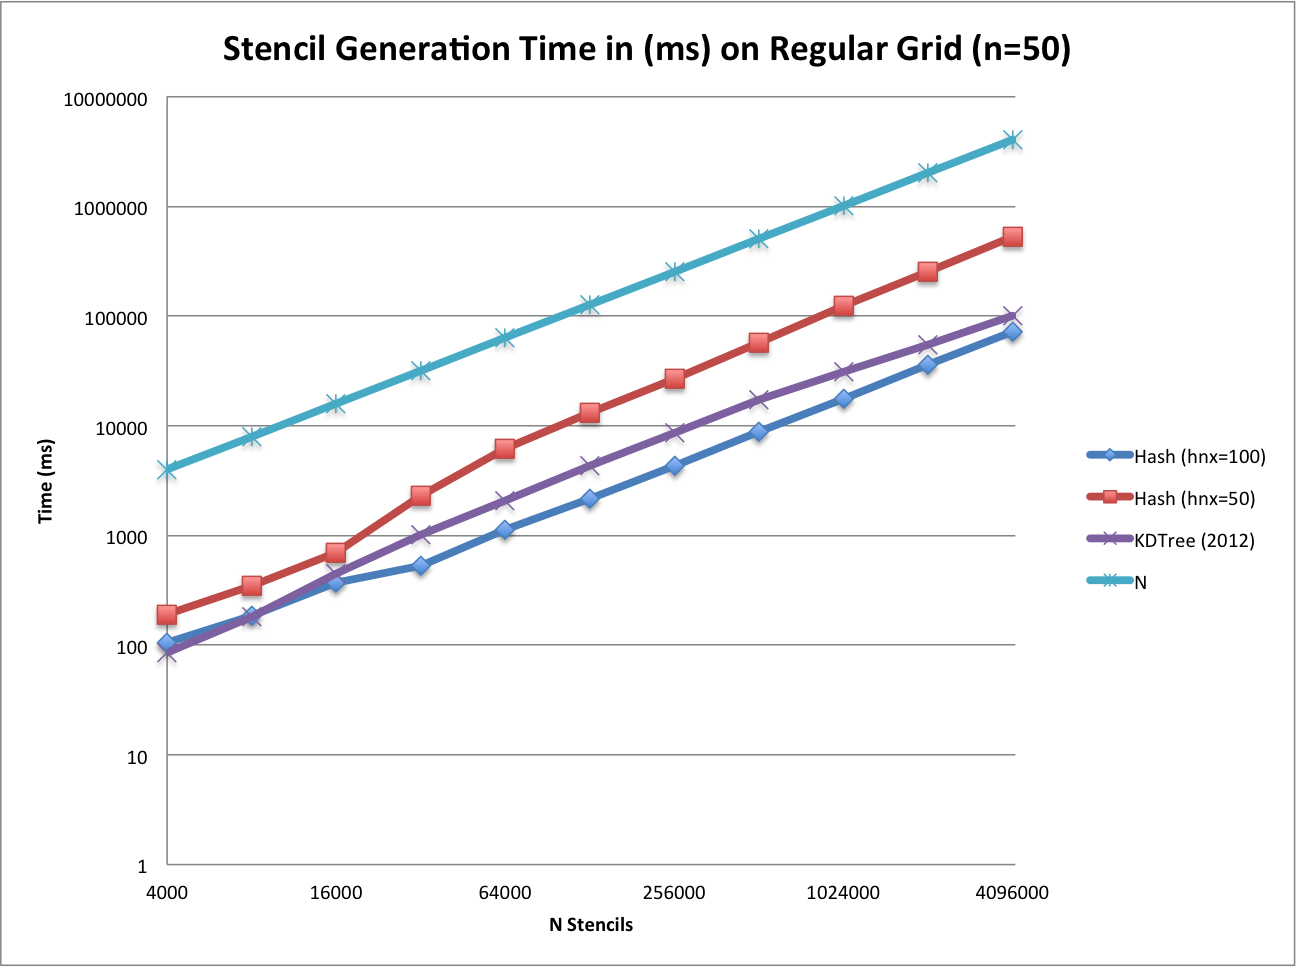
\includegraphics[width=9.5cm]{../figures/stencils/reg_subsets_4m_stencil_gen_time.png}
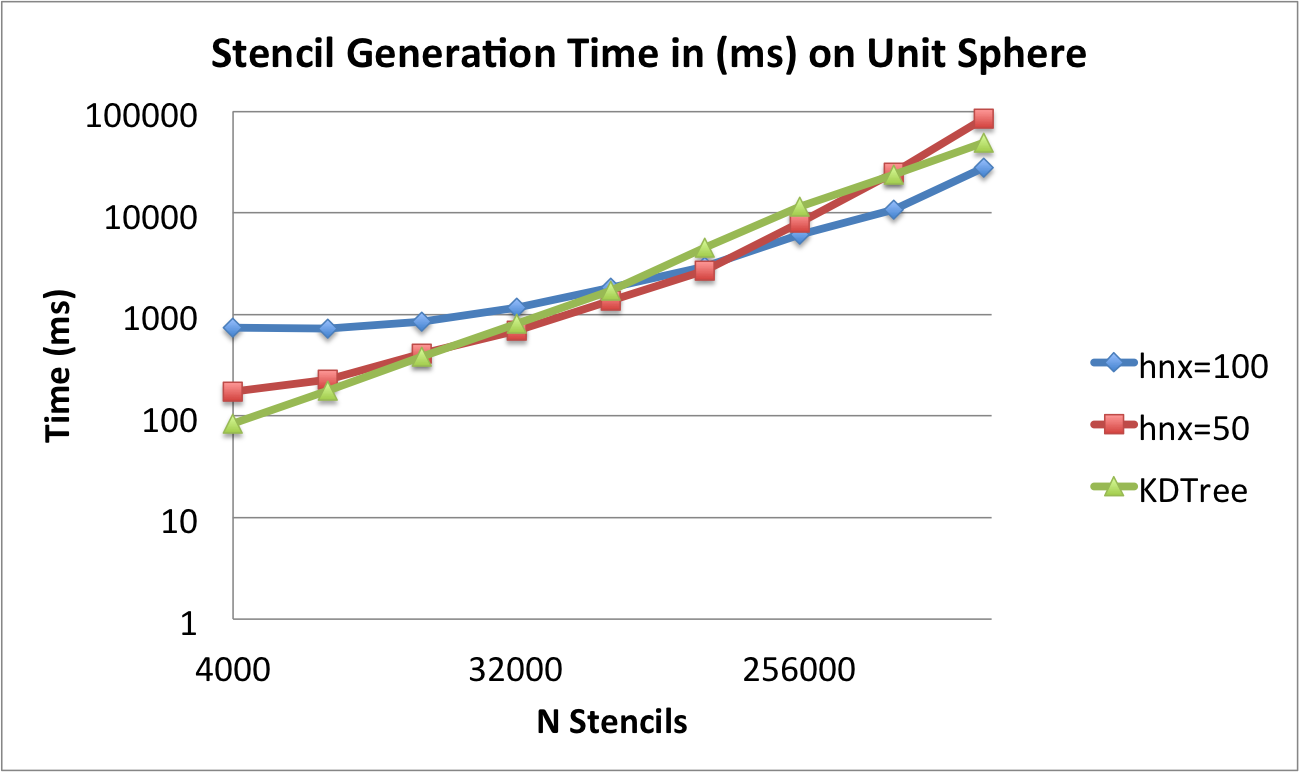
\includegraphics[width=9.5cm]{../figures/stencils/sphere_subsets_1m_stencil_gen_time.png}
\caption{Querying the $n=50$ nearest neighbors on a regular grid up to $N=160^3$ demonstrates the significant gains achieved by our spatially binned neighbor query. While KDTree queries grow as $O(N log N)$}
\label{fig:hash_results}
\end{figure}


The early implementation of $k$-D tree had an $O(n^2)$ growth in complexity. This algorithm was developed to alleviate that cost. It took a few hours to implement but has had some surprising impacts. Note that the complexity of $k$-D tree was reduced to $O(N \log^2 N)$ in 2012. On a regular grid (generated with raster/IJK ordering), the cost of $k$-D tree grows at the same rate as the hashing method. 

At $N=32000$ the cost of hashing drops below $k$-D Tree due to the decreasing number of empty hash cells. Likewise, at $N=1000000$ and beyond, the gap between hashing and $k$-D Tree begins to close as cells contain more than one 


Q: why does the curve drop for $hnx=100$? 
Q: the complexity of the algorithm? 
Q: the sphere I understand: its localizing the search to small patches on the sphere, and 


%TODO: if we overrefine the fixed-grid then the query complexity $\log h_n > \log N$, so the fixed-grid method again starts to lose ground on the $k$-D Tree.


\begin{figure}
\centering
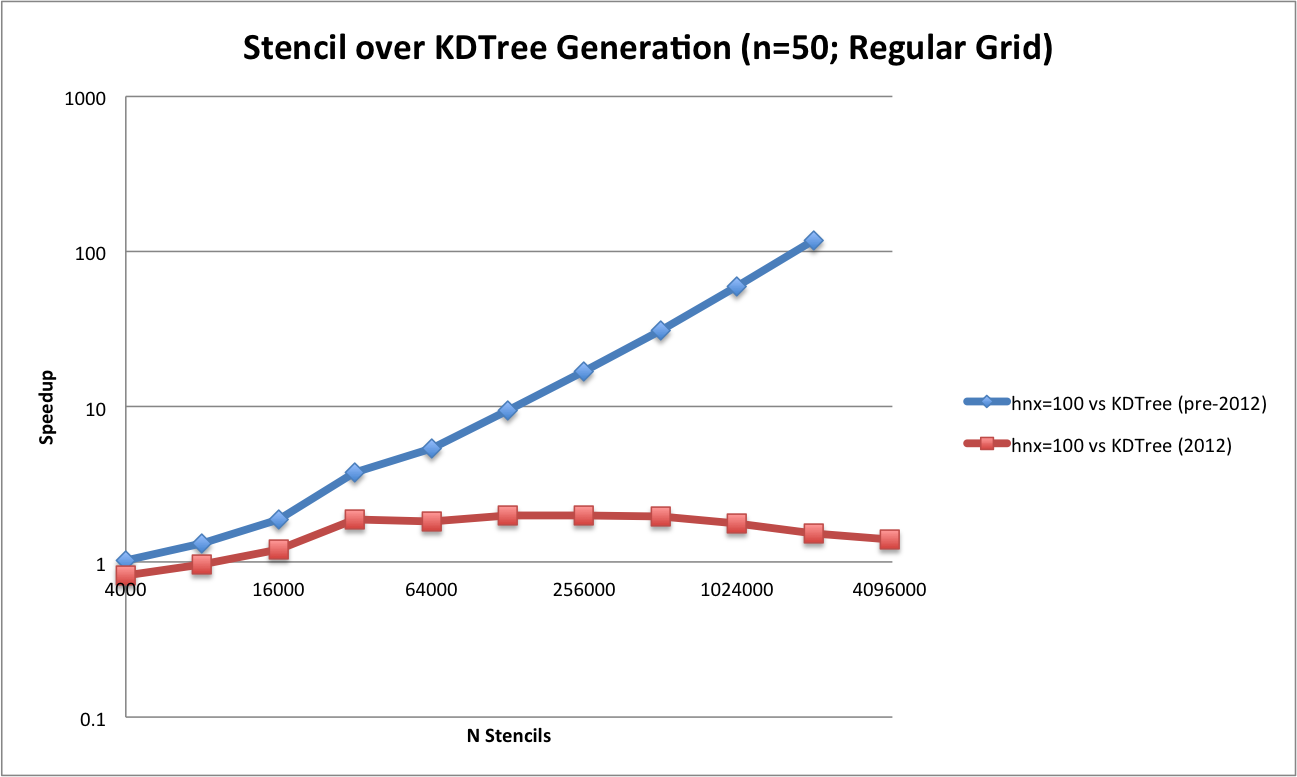
\includegraphics[width=9.5cm]{../figures/stencils/kdtree_old_reg_subsets_4m_stencil_gen_speedup.png}
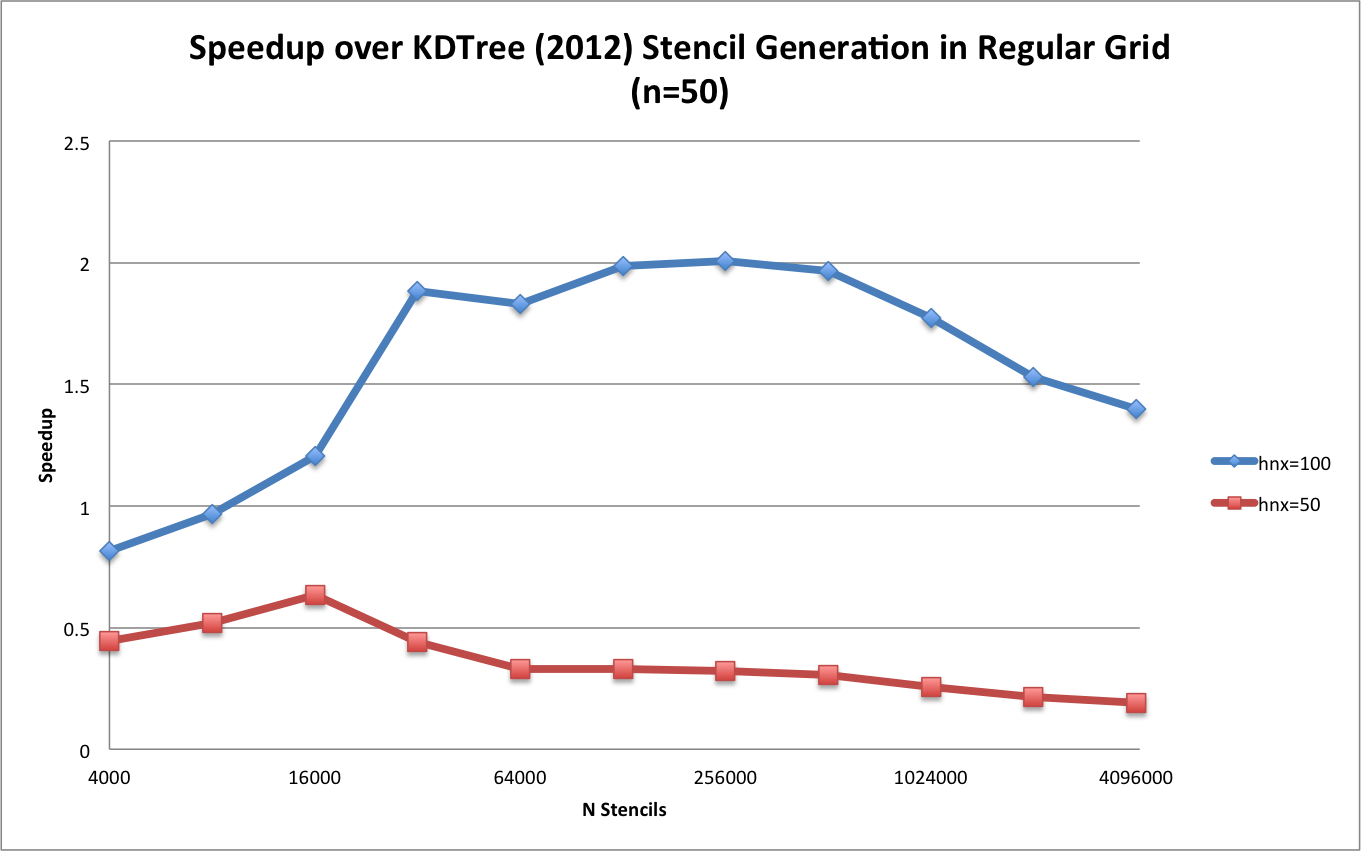
\includegraphics[width=9.5cm]{../figures/stencils/reg_subsets_4m_stencil_gen_speedup.png}
\caption{Querying the $n=50$ nearest neighbors on a regular grid up to $N=160^3$ demonstrates the significant gains achieved by our spatially binned neighbor query. While KDTree queries grow as $O(N log N)$}
\label{fig:hash_results}
\end{figure}
\begin{figure}
\centering
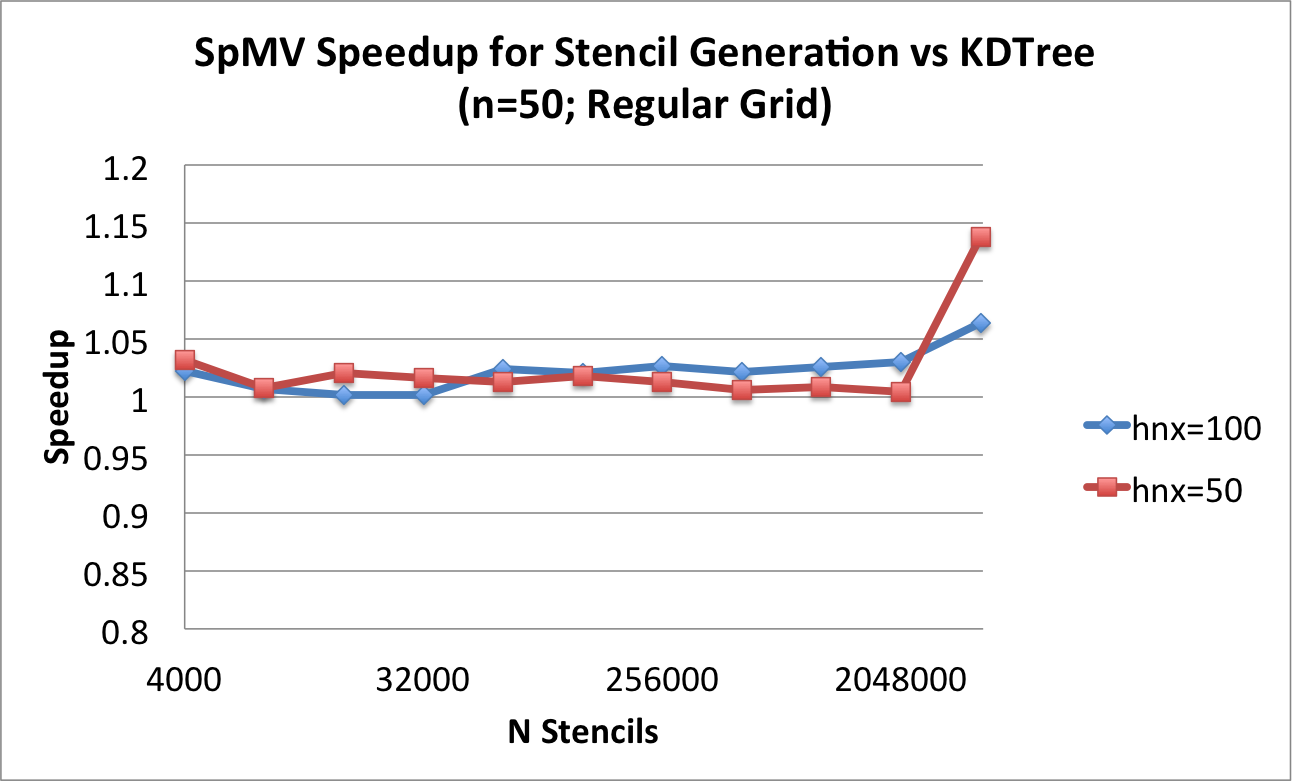
\includegraphics[width=9.5cm]{../figures/stencils/reg_subsets_4m_spmv_speedup.png}
\caption{Querying the $n=50$ nearest neighbors on a regular grid up to $N=160^3$ demonstrates the significant gains achieved by our spatially binned neighbor query. While KDTree queries grow as $O(N log N)$}
\label{fig:hash_results}
\end{figure}
\begin{figure}
\centering
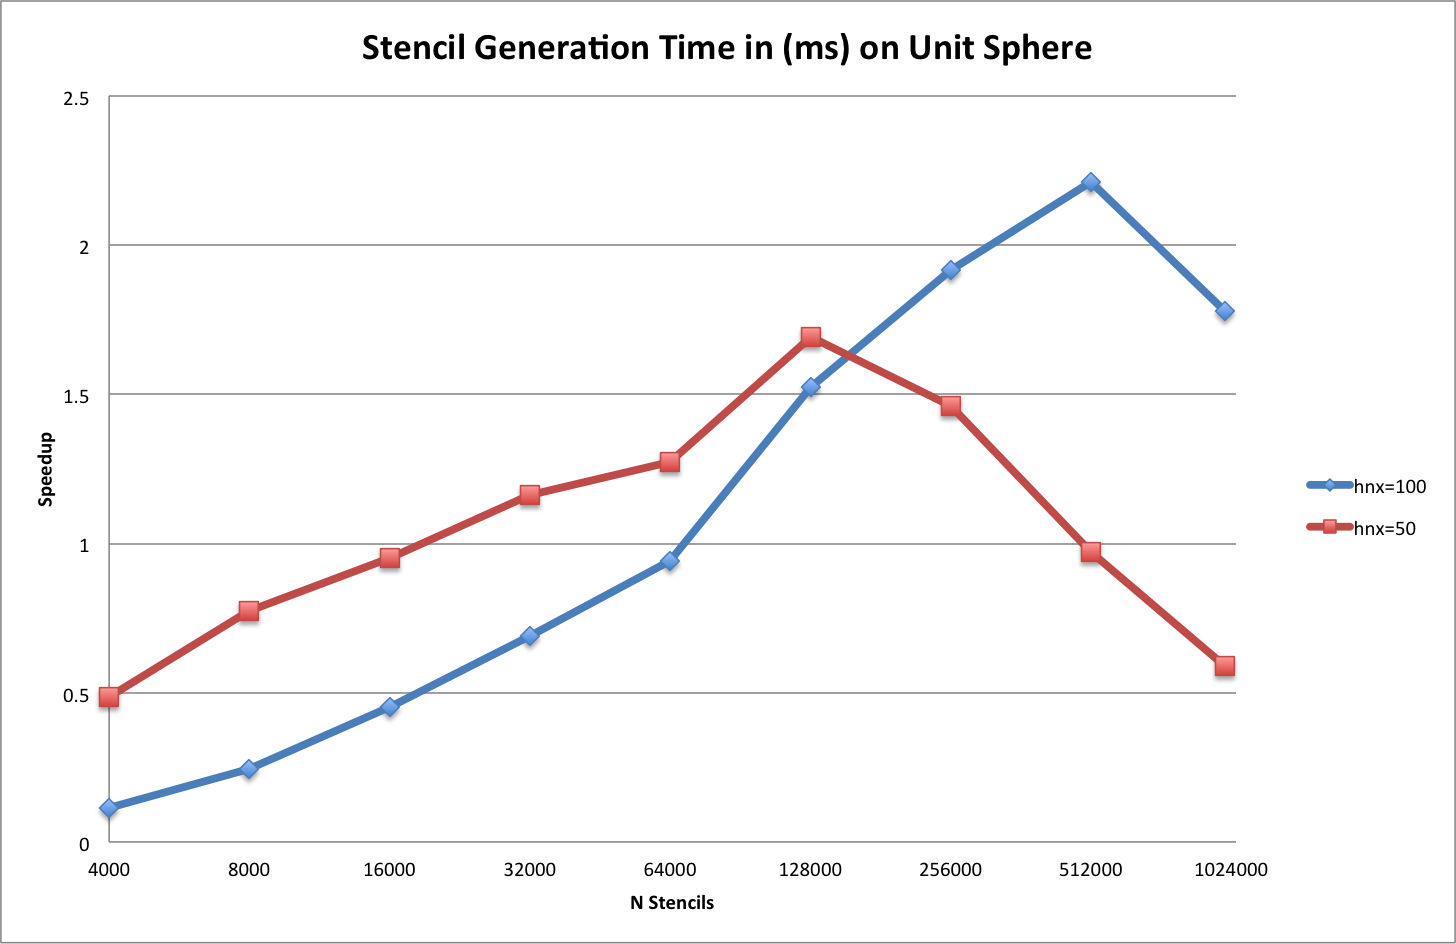
\includegraphics[width=7.5cm]{../figures/stencils/sphere_subsets_1m_stencil_gen_speedup.png}
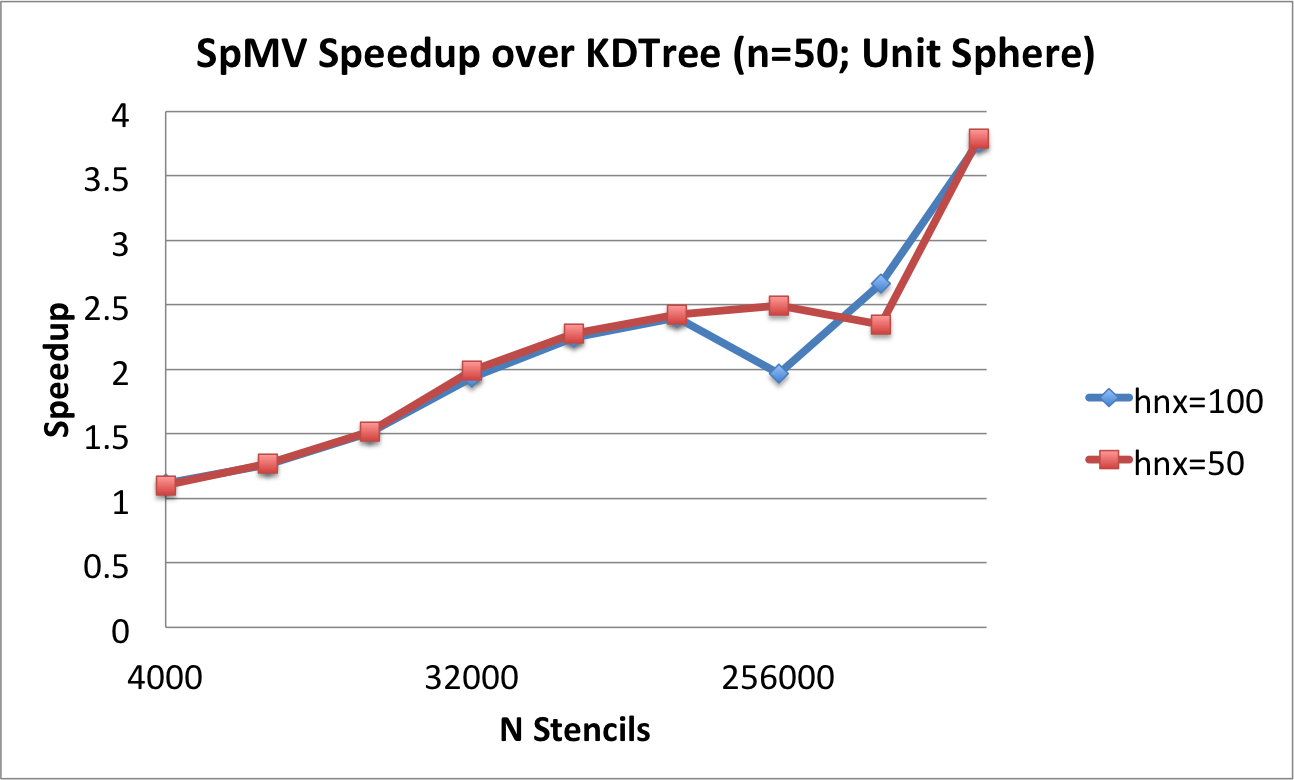
\includegraphics[width=7.5cm]{../figures/stencils/sphere_subsets_1m_spmv_speedup.png}
\caption{Generating stencils for increasing subsets of the $N=1e6$ CVT nodes mesh.}
\label{fig:hash_results}
\end{figure}
\begin{figure}
\centering
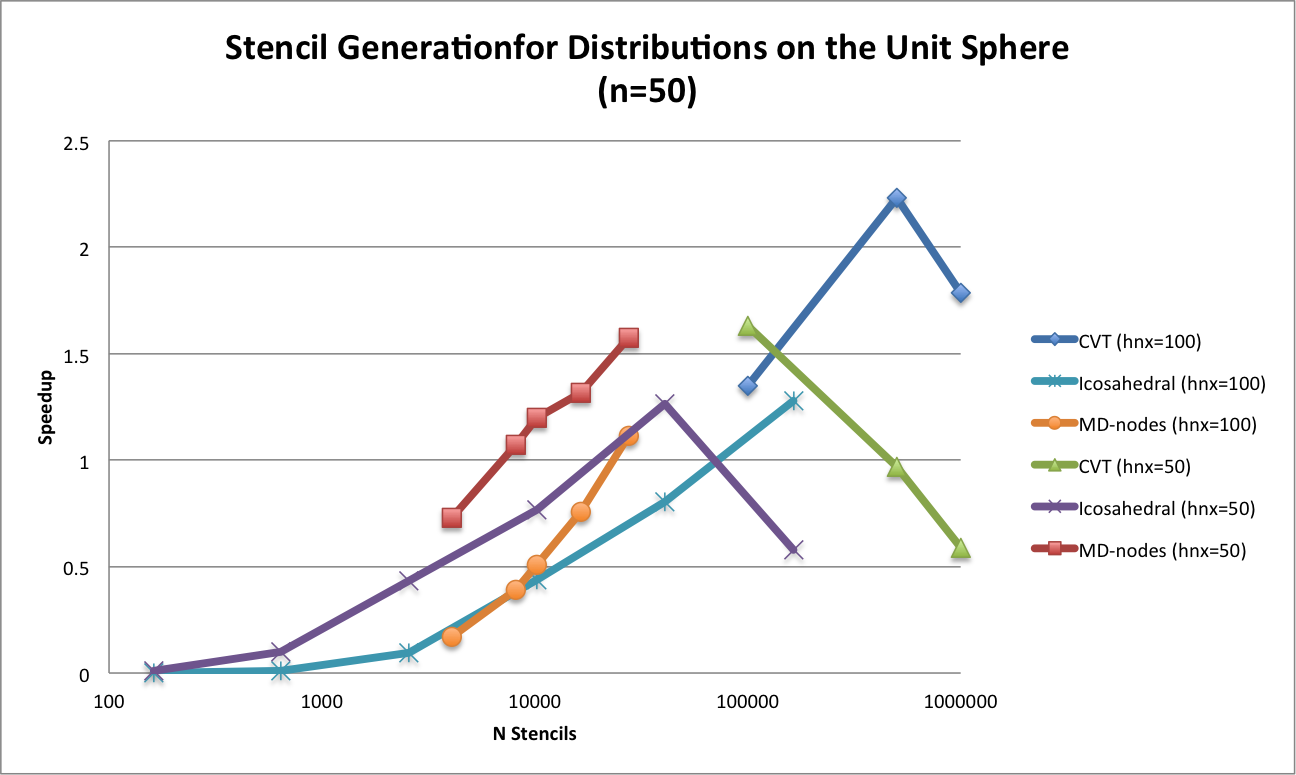
\includegraphics[width=10.5cm]{../figures/stencils/sphere_stencil_gen_speedup.png}
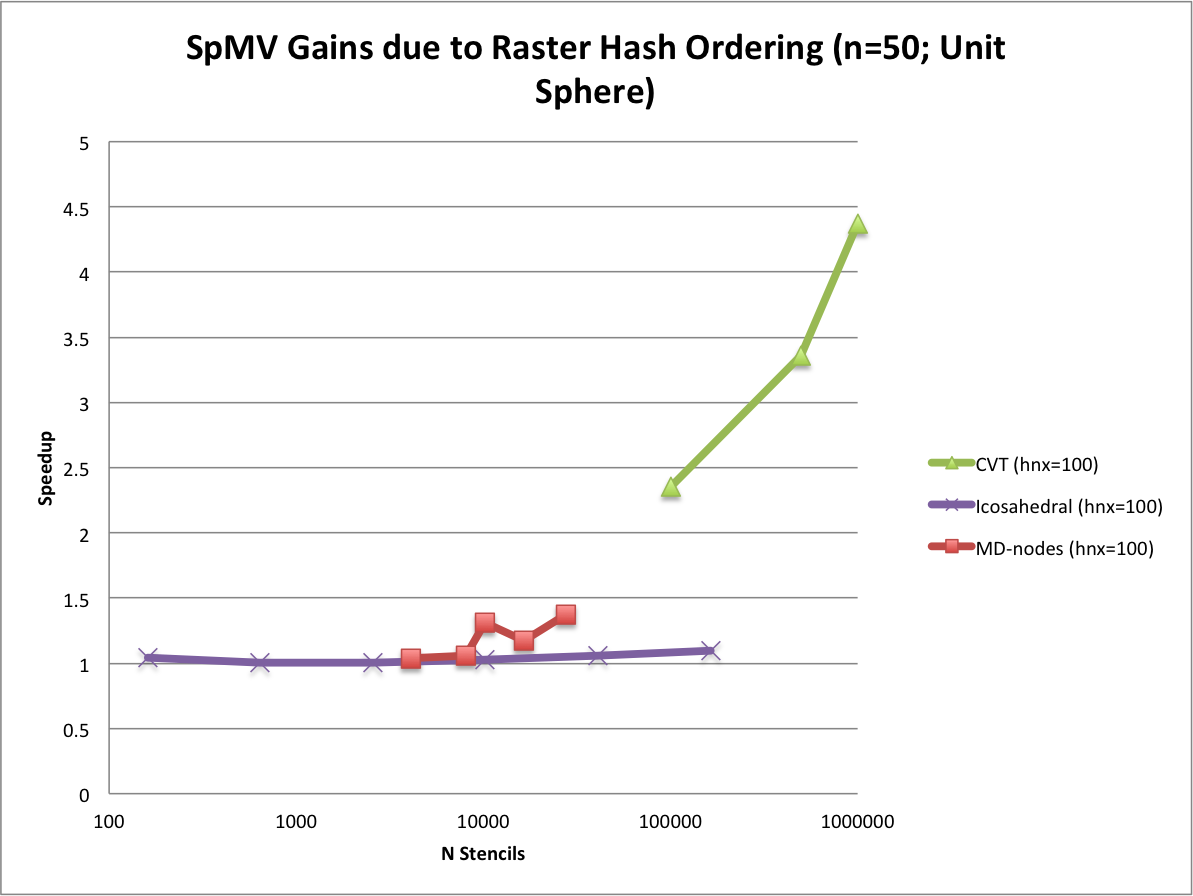
\includegraphics[width=10.5cm]{../figures/stencils/sphere_spmv_speedup.png} 
\caption{Based on the proper choice of overlay resolution, the hash stencil query can accelerate stencil generation, but the sophistication of the algorithm is low enough that negative impact is more likely. On the other hand, the impact on SpMV performance is always positive with the routine accelerated up to 4.9x faster.}
\label{fig:hash_results}
\end{figure}


%TODO: add function for N=1e5, 1e4 to see as a function of N and hnx. 
\begin{figure}
\centering
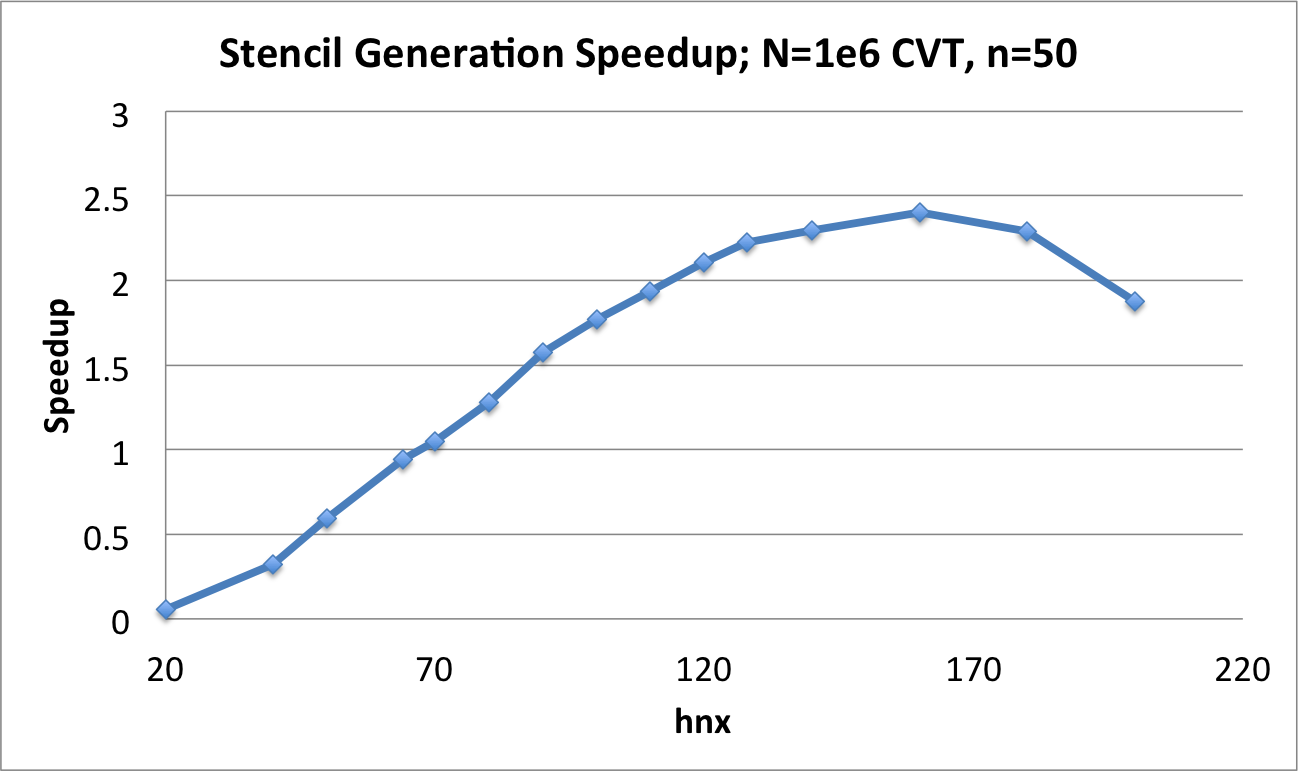
\includegraphics[width=7.5cm]{../figures/stencils/cvt1m_stencil_gen_speedup.png}
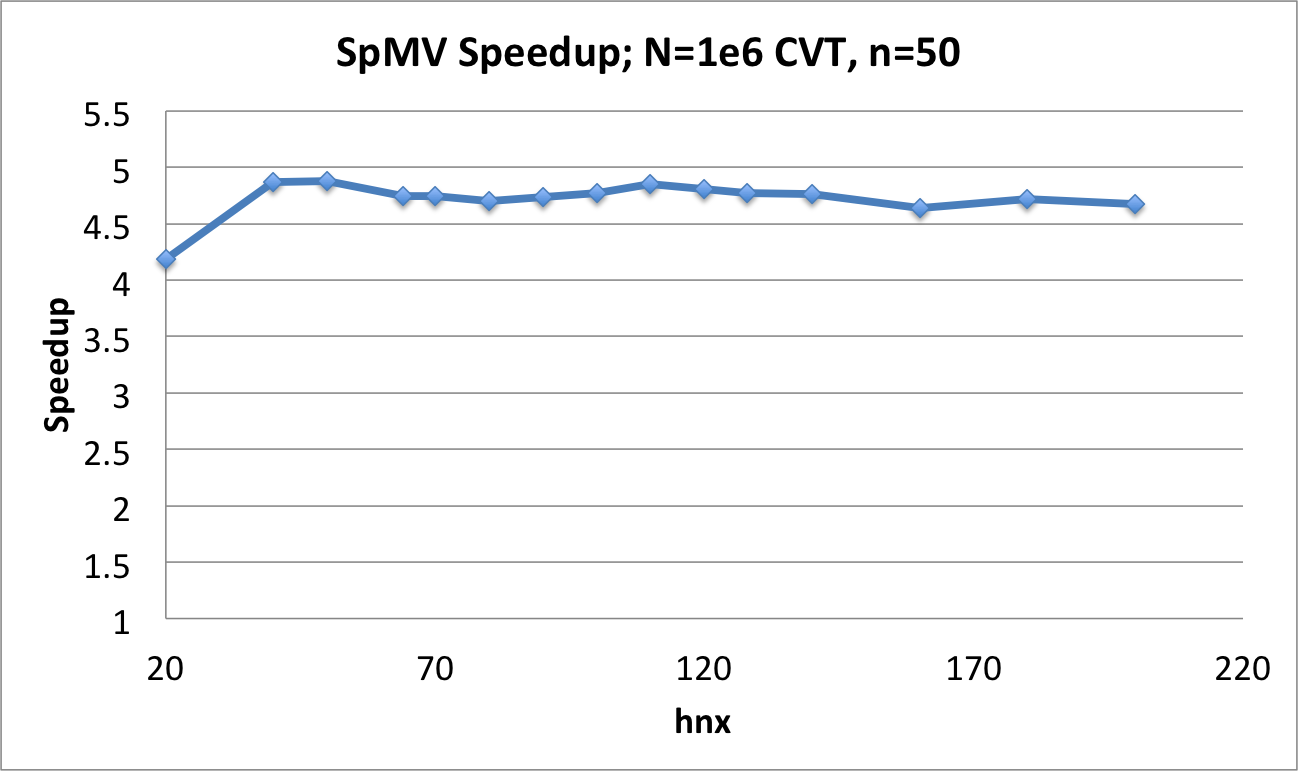
\includegraphics[width=7.5cm]{../figures/stencils/cvt1m_spmv_speedup.png} 
\caption{As the coarse grid resolution increases the hashing algorithm achieves both 2x faster than KDTree in stencil generation, with greater than 4x gain in SpMV performance (for free).}
\label{fig:hash_results}
\end{figure}

For every $N$ there is an optimal $hnx$. This is depicted for $N=500000$ CVT and $hnx=100$. 









\subsection{Alternative Orderings}

%TODO: bandwidth definition
%TODO: dilation for orderings
%TODO: maximum number of cells that we can reorder given 64-bit integer. 

As mentioned, the choice of space filling curve can impact the sparsity pattern of differentiation matrices. Those patterns in turn correlate to differenct memory access patterns

 Examples include $Z$- or \emph{Morton} ordering, $U$- or \emph{Greycode}-ordering, $X$-ordering, etc. Hilbert curves have been demonstrated to be the most efficient \cite{INREFS}. 

The authors of \cite{Goswami2010} utilize $Z$-ordering in their 


The ideal differentiation matrix, corresponding to discretization of a line, would have all non-zeros on the first $\frac{n-1}{2}$ to each side of the diagonal. For 2- or 3-D domains the ideal case is not possible to achieve, but the nodes can be reordered with the goal to condense
At the end of BuildFixedGrid the original set of nodes, $P$ is overwritten by $\hat{P}$. While nothing requires that $\hat{P}$ replace the usage of $P$ 



\cite{MellorCrummey2001} found that reodering nodes via RCM and space filling curves offer similar benefits in terms of reduced TLB misses and better cache coherency. 



\subsubsection{Cuthill-McKee} 


The Cuthill McKee algorithms can be equated to a breadth-first search. The algorithm queues nodes in order of degree at each level of the search and traverses the lowest degree priority. The Reverse variant of Cuthill-McKee inverts the node order so that the lowest degree and top level node are at the end of the matrix rather than the beginning. Aside from ordering, the Reverse and Standard Cuthill McKee algorithms are identical processes. RCM is the more popular of the variants though, due to storage savings and reduced fill-in for some decompositions \cite{LiuSherman1976}.






\subsection{Impact of Orderings}


Rather than complete a full analysis of the impact from space filling curves, we only consider the ideal cases from CVT and RG (because they are used in the thesis). The integer dilation is costly and does not appear to significantly improve the performance of the best cases.

RCM is effective and used with KDTree. 



\begin{figure}
\centering
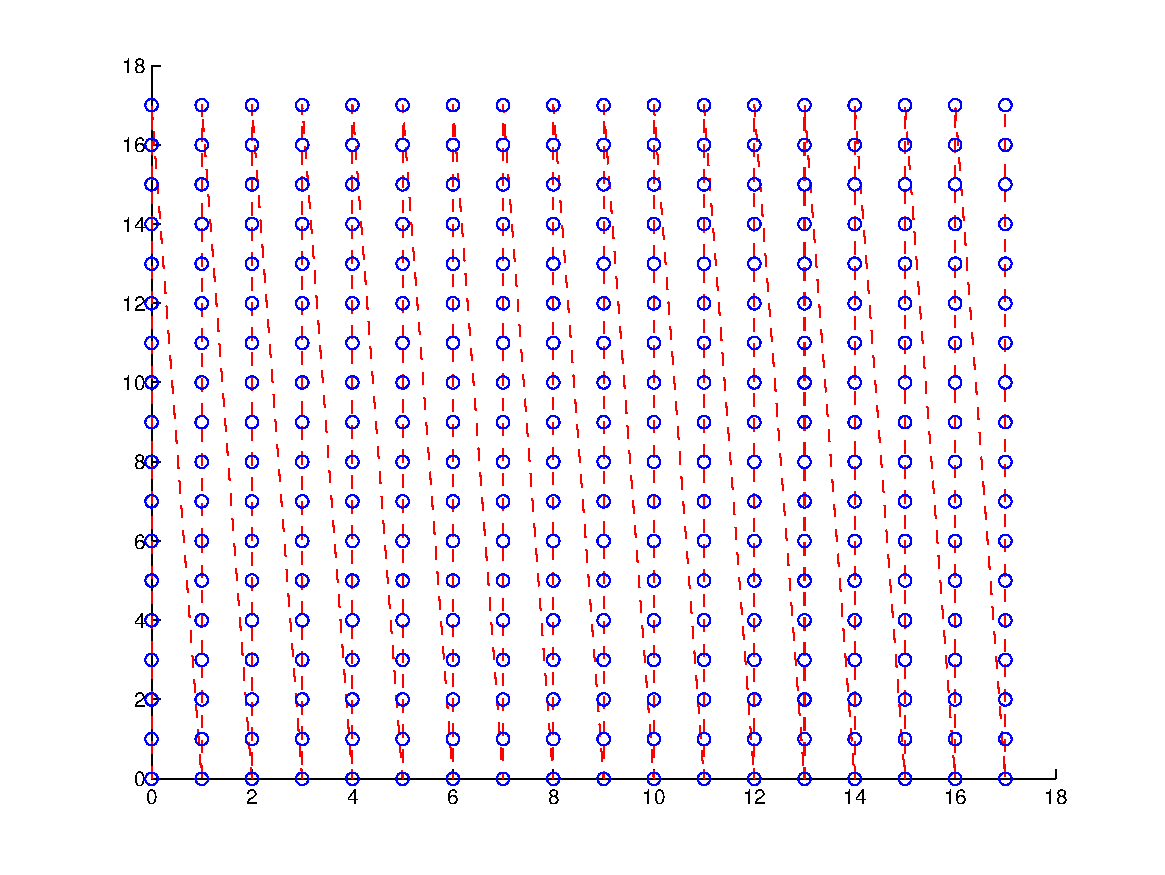
\includegraphics[width=0.45\textwidth]{rbffd_methods_content/hashing/originalorder_regulargrid-eps-converted-to.pdf}
\caption{In order: a) node ordering test cases; b) original ordering of regular grid (raster); c) coarse grid overlay for hash functions ($hnx = 6$); d) example stencil ($n=31$) spanning multiple Z's; e) spy of DM after orderings. \authnote{REGENERATE FIGURES WITH RANDOM/HALTON NODES}}
\label{fig:orderings}
\end{figure}

\begin{figure}
\centering
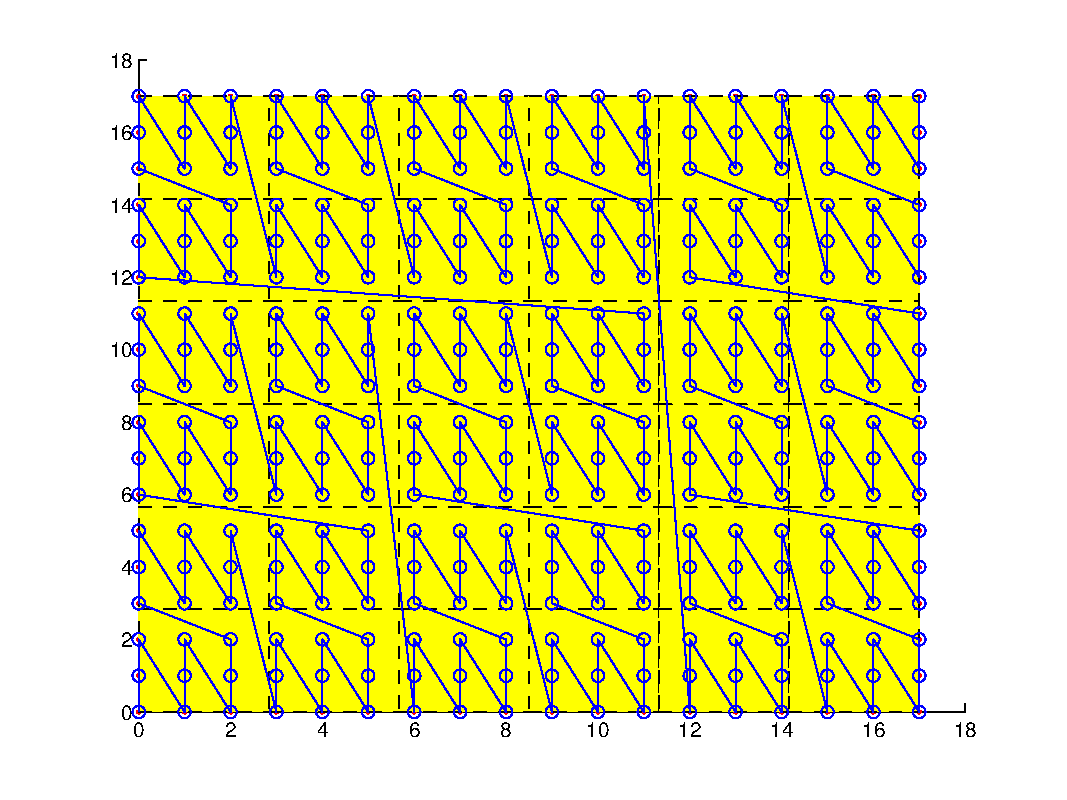
\includegraphics[width=0.45\textwidth]{rbffd_methods_content/hashing/overlay_regulargrid-eps-converted-to.pdf} 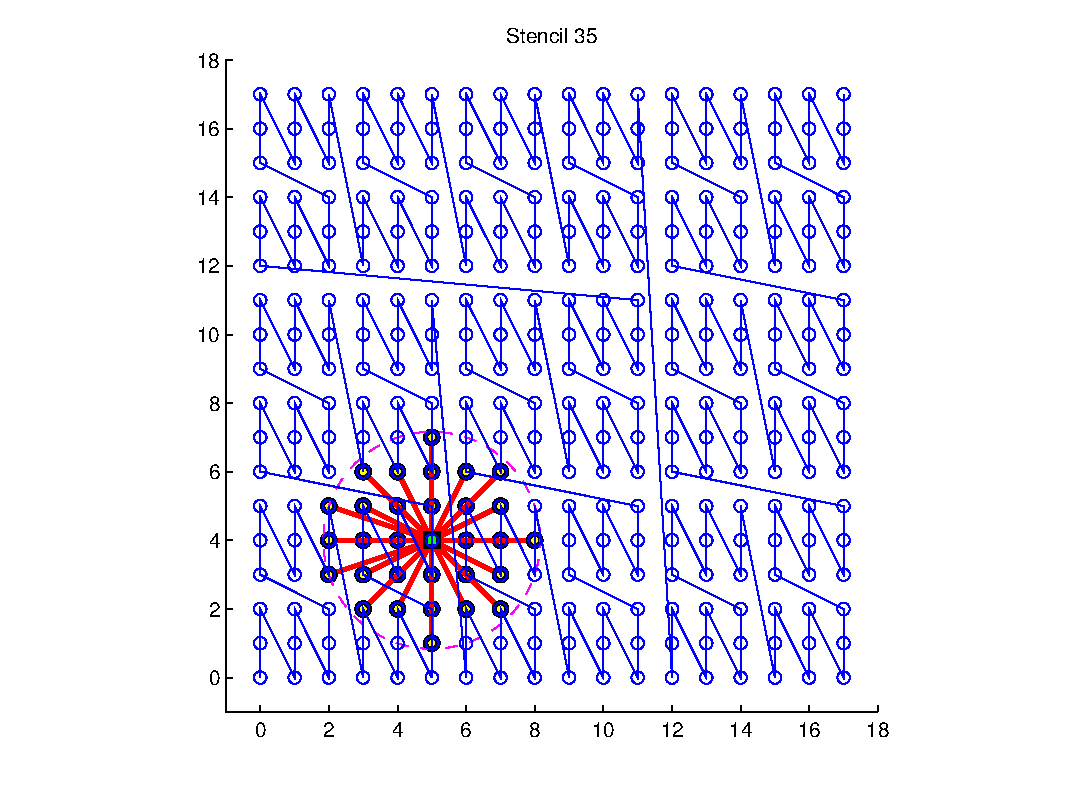
\includegraphics[width=0.45\textwidth]{rbffd_methods_content/hashing/stencil_regulargrid-eps-converted-to.pdf}
\caption{In order: a) node ordering test cases; b) original ordering of regular grid (raster); c) coarse grid overlay for hash functions ($hnx = 6$); d) example stencil ($n=31$) spanning multiple Z's; e) spy of DM after orderings. }
\label{fig:orderings}
\end{figure}

Obviously, the ideal case for bandwidth is when all rows contain the $\frac{n}{2}$ nodes corresponding to solution value to either side of $u_j$. In 1-D this corresponds to every node containing the $\frac{n}{2}$ nodes to the left and right of $x_j$. In 2-D this is only possible if the nodes in the domain are properly indexed such that stencils contain the proper set of neighbors---a stringent requirement that will 

impact from ordering on matrix sparsity. Bandwidth impact. Bandwidth impact on condition considered in future chapter. 

One frequently hears that ordering via space filling curves like Morton Ordering and/or gray codes can benefit memory access patterns. 

(Related? \url{http://publish.uwo.ca/~shaque4/presentationSONAD.pdf} \url{http://www.cs.duke.edu/~alvy/papers/sc98/} \url{http://www.cs.indiana.edu/~dswise/Arcee/Papers/medea06.pdf} \url{http://citeseerx.ist.psu.edu/viewdoc/download?doi=10.1.1.118.7720&rep=rep1&type=pdf} \url{http://stackoverflow.com/questions/4260002/benefits-of-nearest-neighbor-search-with-morton-order})

\section{Conclusion and Future Work}



%TODO: move down
Although RBF-FD only requires neighbor queries once, the results that follow reveal a long lasting positive impact on memory with a fixed-grid method, which is sufficient to justify its use. Investigations into moving node coordinates and/or local refinements for RBF methods (e.g., \cite{FlyerLehto10}) would find the fixed-grid method significantly more beneficial. As of this writing no known applications of RBF-FD consider moving nodes

Due to the limited significance of stencil generation under RBF-FD, the overhead in implementing and debugging the fixed-grid method on the GPU is difficult to justify. The implementation tested here was developed as a pure CPU prototype with minimal attention to optimization. The added complexity in reproducing the efficient fixed-grid method on the GPU could be the subject of future work for moving nodes. 

\cite{Connor2009} could benefit the algorithm by sorting nodes completely based on floating point $Z$-ordering.




\subsection{Future Work}

The complexity of the method is still higher than the more efficient implementations used by Lagrangian methods, but as demonstrated in Figure~\ref{sten_methods_compare} the savings are significant. Generating stencils for RBF-FD is a preprocessing cost, so we do not dedicate an excessive amount of attention to this algorithm. However, a few ideas that would improve: hilbert ordering, choose AABB resolution based on $N$ not user parameters, faster sorting, GPU implementation

Open item from to this section include: 
\begin{itemize} 
\item An efficient GPU $k$-NN implementation for the investigation of RBF-FD in a moving nodes or adaptive mesh refinement situation. Examples include \cite{Pan2011, Goswami2010, Connor2009, Brown2010}
\item Space filling curves are limited to a MATLAB prototype at the moment. These can be implemented in C++ for integers, with a potential investigation into floating point dilation and orderings \cite{Connor2009}.
\item 
\end{itemize}

\cite{Saad2003} mentions the impact of ordering on conditioning.




%TODO: add RCM and fix order
\begin{figure}
\centering
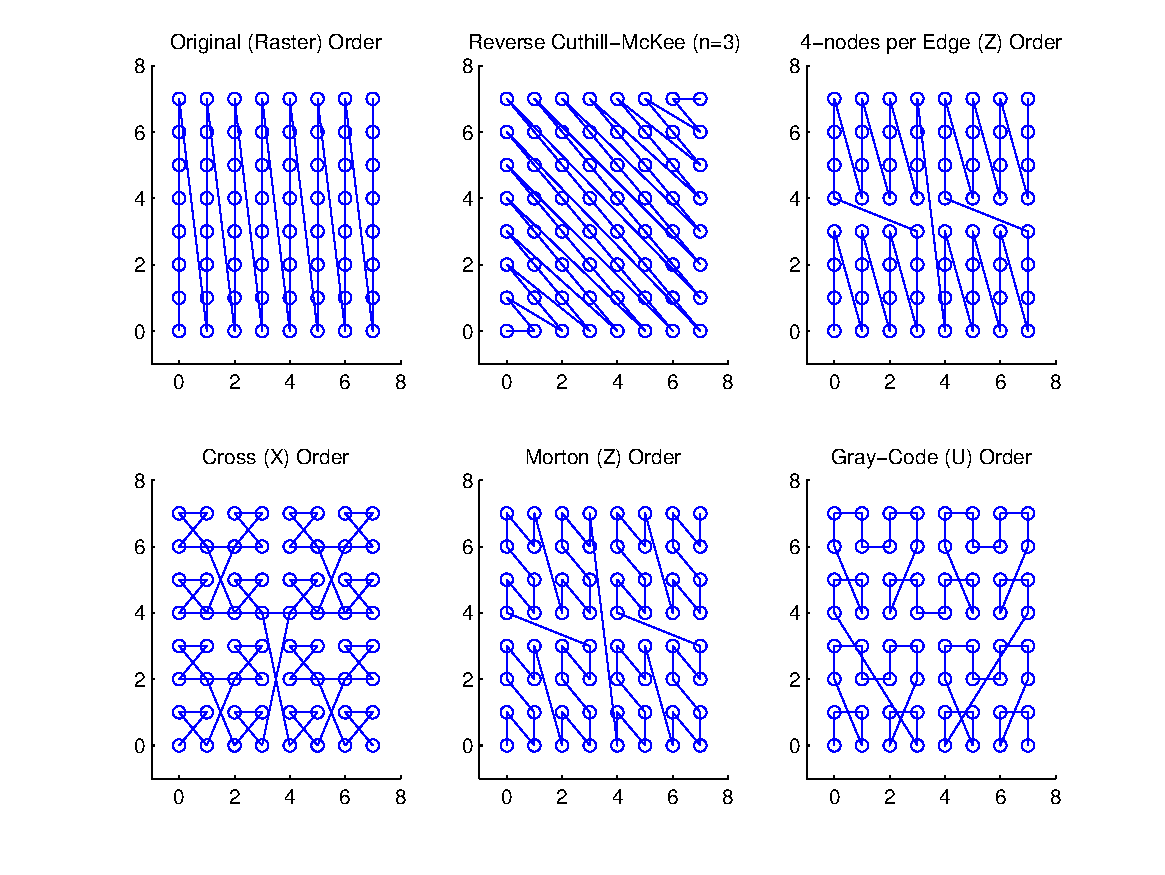
\includegraphics[width=\textwidth]{rbffd_methods_content/hashing/node_orderings-eps-converted-to.pdf} \\
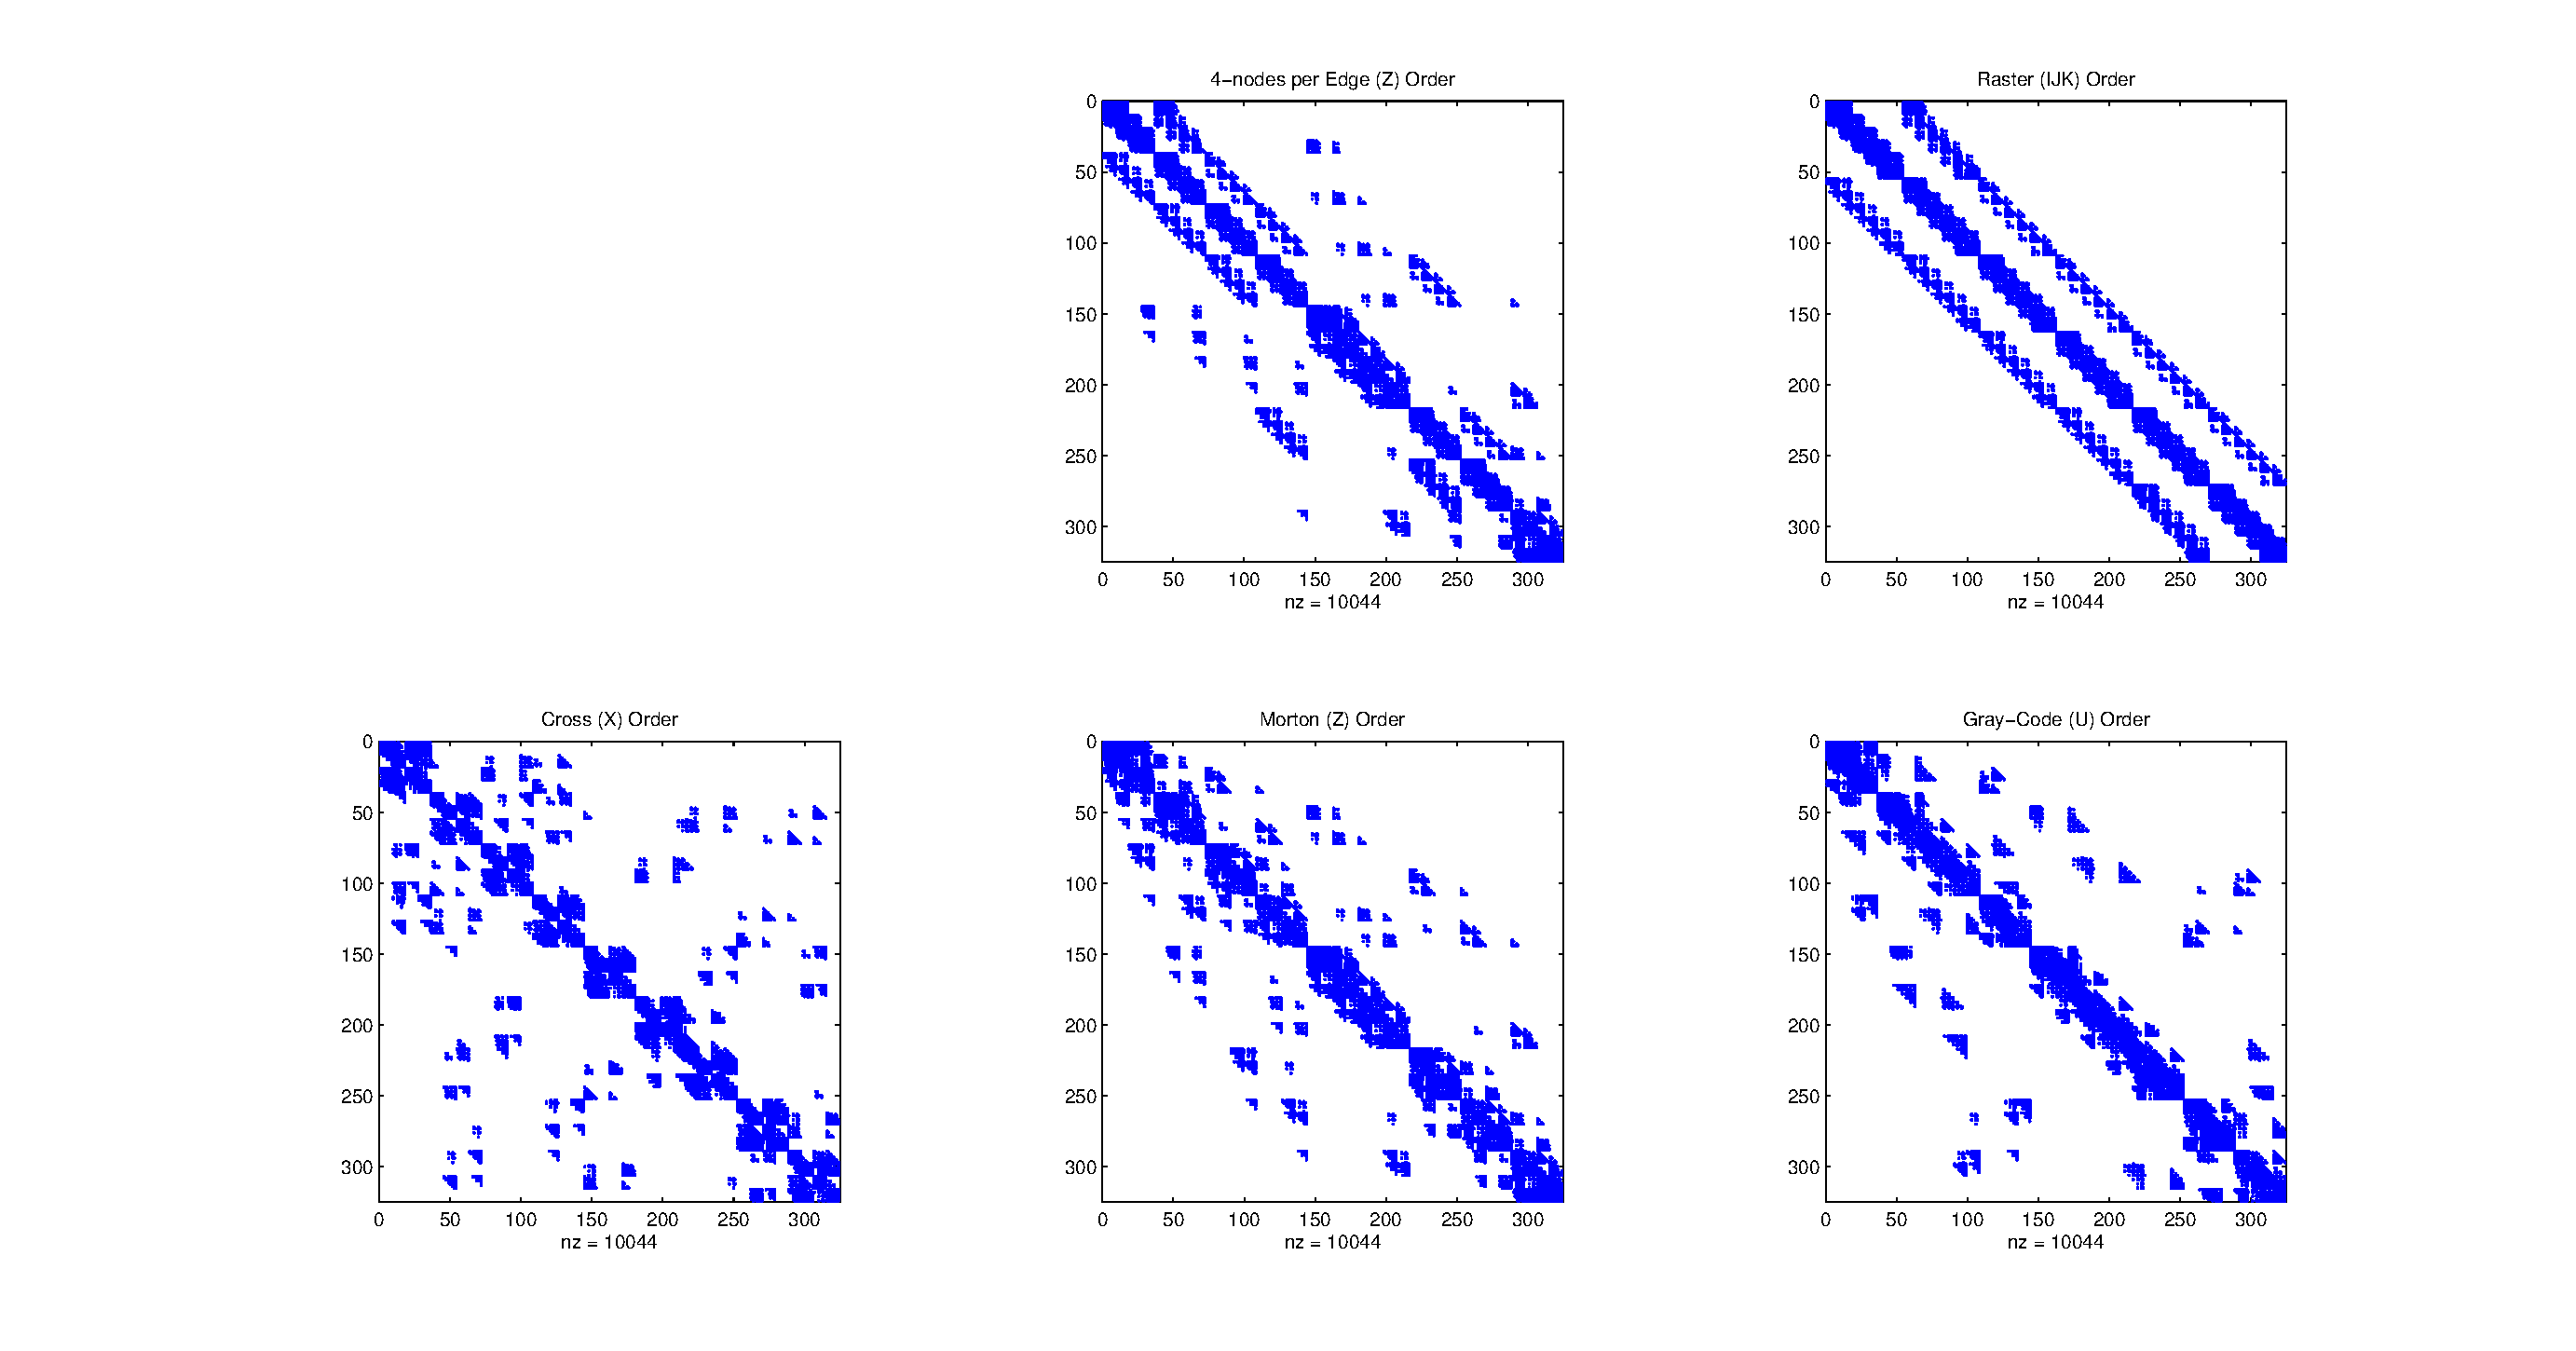
\includegraphics[width=\textwidth]{rbffd_methods_content/hashing/spy_regulargrid-eps-converted-to.pdf} 
\caption{In order: a) node ordering test cases; b) original ordering of regular grid (raster); c) coarse grid overlay for hash functions ($hnx = 6$); d) example stencil ($n=31$) spanning multiple Z's; e) spy of DM after orderings. \authnote{TODO: Raster on top left. Add RCM ordering to top right.}  }
\label{fig:orderings}
\end{figure}


\section{Conclusions on Stencil Generation}

For quasi-regular distributions and small to medium sized grids the $k$-D Tree performs well enough in comparison to the fixed-grid method. However, the difference in 
%TODO: what value? 

There is an ideal $h_n$. %TODO: what is is as a function of N?


\ifstandalone
\bibliographystyle{plain}
\bibliography{merged_references}
\end{document}
\else
\expandafter\endinput
\fi
